%----------
%   IMPORTANTE
%----------

% Si nunca has utilizado LaTeX es conveniente que aprendas una serie de conceptos básicos antes de utilizar esta plantilla. Te aconsejamos que leas previamente algún tutorial (puedes encontar muchos en Internet).

% Esta plantilla está basada en las recomendaciones de la guía "Trabajo fin de Máster: Escribir el TFM", que encontrarás en http://uc3m.libguides.com/TFM/escribir
% contiene recomendaciones de la Biblioteca basadas principalmente en estilos APA e IEEE, pero debes seguir siempre las orientaciones de tu Tutor de TFM y la normativa de TFM para tu titulación.

% Encontrarás un ejemplo de TFM realizado con esta misma plantilla en la carpeta "_ejemplo_TFM_2019". Consúltalo porque contiene ejemplos útiles para incorporar tablas, figuras, listados de código, bibliografía, etc.


%----------
%	CONFIGURACIÓN DEL DOCUMENTO
%----------

% Definimos las características del documento y añadimos una serie de paquetes (\usepackage{package}) que agregan funcionalidades a LaTeX.

\documentclass[12pt]{report} %fuente a 12pt

% MÁRGENES: 2,5 cm sup. e inf.; 3 cm izdo. y dcho.
\usepackage[
a4paper,
vmargin=2.5cm,
hmargin=3cm
]{geometry}

% INTERLINEADO: Estrecho (6 ptos./interlineado 1,15) o Moderado (6 ptos./interlineado 1,5)
\renewcommand{\baselinestretch}{1.15}
\parskip=6pt

% DEFINICIÓN DE COLORES para portada y listados de código
\usepackage[table]{xcolor}
\definecolor{azulUC3M}{RGB}{0,0,102}
\definecolor{gray97}{gray}{.97}
\definecolor{gray75}{gray}{.75}
\definecolor{gray45}{gray}{.45}

% Soporte para GENERAR PDF/A --es importante de cara a su inclusión en e-Archivo porque es el formato óptimo de preservación y a la generación de metadatos, tal y como se describe en http://uc3m.libguides.com/ld.php?content_id=31389625. En la carpeta incluímos el archivo plantilla_tfg_2017.xmpdata en el que puedes incluir los metadatos que se incorporarán al archivo PDF cuando lo compiles. Ese archivo debe llamarse igual que tu archivo .tex. Puedes ver un ejemplo en esta misma carpeta.
\usepackage[a-1b]{pdfx}

% ENLACES
\usepackage{hyperref}
\hypersetup{colorlinks=true,
	linkcolor=black, % enlaces a partes del documento (p.e. índice) en color negro
	urlcolor=blue} % enlaces a recursos fuera del documento en azul

% EXPRESIONES MATEMATICAS
\usepackage{amsmath,amssymb,amsfonts,amsthm}
\usepackage{subcaption}
\usepackage{txfonts} 
\usepackage[T1]{fontenc}
\usepackage[utf8]{inputenc}

\usepackage[english]{babel} 
\usepackage[babel, english=american]{csquotes}
\AtBeginEnvironment{quote}{\small}

% diseño de PIE DE PÁGINA
\usepackage{fancyhdr}
\pagestyle{fancy}
\fancyhf{}
\renewcommand{\headrulewidth}{0pt}
\rfoot{\thepage}
\fancypagestyle{plain}{\pagestyle{fancy}}

% DISEÑO DE LOS TÍTULOS de las partes del trabajo (capítulos y epígrafes o subcapítulos)
\usepackage{titlesec}
\usepackage{titletoc}
\titleformat{\chapter}[block]
{\large\bfseries\filcenter}
{\thechapter.}
{5pt}
{\MakeUppercase}
{}
\titlespacing{\chapter}{0pt}{0pt}{*3}
\titlecontents{chapter}
[0pt]                                               
{}
{\contentsmargin{0pt}\thecontentslabel.\enspace\uppercase}
{\contentsmargin{0pt}\uppercase}                        
{\titlerule*[.7pc]{.}\contentspage}                 

\titleformat{\section}
{\bfseries}
{\thesection.}
{5pt}
{}
\titlecontents{section}
[5pt]                                               
{}
{\contentsmargin{0pt}\thecontentslabel.\enspace}
{\contentsmargin{0pt}}
{\titlerule*[.7pc]{.}\contentspage}

\titleformat{\subsection}
{\normalsize\bfseries}
{\thesubsection.}
{5pt}
{}
\titlecontents{subsection}
[10pt]                                               
{}
{\contentsmargin{0pt}                          
	\thecontentslabel.\enspace}
{\contentsmargin{0pt}}                        
{\titlerule*[.7pc]{.}\contentspage}  


% DISEÑO DE TABLAS. Puedes elegir entre el estilo para ingeniería o para ciencias sociales y humanidades. Por defecto, está activado el estilo de ingeniería. Si deseas utilizar el otro, comenta las líneas del diseño de ingeniería y descomenta las del diseño de ciencias sociales y humanidades
\usepackage{multirow} %permite combinar celdas 
\usepackage{caption} %para personalizar el título de tablas y figuras
\usepackage{floatrow} %utilizamos este paquete y sus macros \ttabbox y \ffigbox para alinear los nombres de tablas y figuras de acuerdo con el estilo definido. Para su uso ver archivo de ejemplo 
\usepackage{array} % con este paquete podemos definir en la siguiente línea un nuevo tipo de columna para tablas: ancho personalizado y contenido centrado
\newcolumntype{P}[1]{>{\centering\arraybackslash}p{#1}}
\DeclareCaptionFormat{upper}{#1#2\uppercase{#3}\par}

% Diseño de tabla para ingeniería
\captionsetup[table]{
	format=upper,
	justification=centering,
	labelsep=period,
	width=.75\linewidth,
	labelfont=small,
	font=small,
}

%Diseño de tabla para ciencias sociales y humanidades
%\captionsetup[table]{
%	justification=raggedright,
%	labelsep=period,
%	labelfont=small,
%	singlelinecheck=false,
%	font={small,bf}
%}


% DISEÑO DE FIGURAS. Puedes elegir entre el estilo para ingeniería o para ciencias sociales y humanidades. Por defecto, está activado el estilo de ingeniería. Si deseas utilizar el otro, comenta las líneas del diseño de ingeniería y descomenta las del diseño de ciencias sociales y humanidades
\usepackage{graphicx}
\graphicspath{{figures/}} %ruta a la carpeta de imágenes

% Diseño de figuras para ingeniería
\captionsetup[figure]{
	format=hang,
	name=Fig.,
	singlelinecheck=off,
	labelsep=period,
	labelfont=small,
	font=small		
}

% Diseño de figuras para ciencias sociales y humanidades
%\captionsetup[figure]{
%	format=hang,
%	name=Figure,
%	singlelinecheck=off,
%	labelsep=period,
%	labelfont=small,
%	font=small		
%}


% NOTAS A PIE DE PÁGINA
\usepackage{chngcntr} %para numeración contínua de las notas al pie
\counterwithout{footnote}{chapter}

% LISTADOS DE CÓDIGO
% soporte y estilo para listados de código. Más información en https://es.wikibooks.org/wiki/Manual_de_LaTeX/Listados_de_código/Listados_con_listings
\usepackage{listings}

% definimos un estilo de listings
\lstdefinestyle{estilo}{ frame=Ltb,
	framerule=0pt,
	aboveskip=0.5cm,
	framextopmargin=3pt,
	framexbottommargin=3pt,
	framexleftmargin=0.4cm,
	framesep=0pt,
	rulesep=.4pt,
	backgroundcolor=\color{gray97},
	rulesepcolor=\color{black},
	%
	basicstyle=\ttfamily\footnotesize,
	keywordstyle=\bfseries,
	stringstyle=\ttfamily,
	showstringspaces = false,
	commentstyle=\color{gray45},     
	%
	numbers=left,
	numbersep=15pt,
	numberstyle=\tiny,
	numberfirstline = false,
	breaklines=true,
	xleftmargin=\parindent
}

\captionsetup[lstlisting]{font=small, labelsep=period}
% fijamos el estilo a utilizar 
\lstset{style=estilo}
\renewcommand{\lstlistingname}{\uppercase{Código}}


%BIBLIOGRAFÍA - PUEDES ELEGIR ENTRE ESTILO IEEE O APA. POR DEFECTO ESTÁ CONFIGURADO IEEE. SI DESEAS USAR APA, COMENTA LAS LÍNEA DE IEEE Y DESCOMENTA LAS DE APA. Si haces cambios en la configuración de la bibliografía y no obtienes los resultados esperados, es recomendable limpiar los archivos auxiliares y volver a compilar en este orden: COMPILAR-BIBLIOGRAFIA-COMPILAR
% Tienes más información sobre cómo generar bibliografía en http://tex.stackexchange.com/questions/154751/biblatex-with-biber-configuring-my-editor-to-avoid-undefined-citations , https://es.sharelatex.com/learn/Bibliography_management_in_LaTeX y en http://www.ctan.org/tex-archive/macros/latex/exptl/biblatex-contrib
% También te recomendamos consultar la guía temática de la Biblioteca sobre citas bibliográficas: http://uc3m.libguides.com/guias_tematicas/citas_bibliograficas/inicio

% CONFIGURACIÓN PARA LA BIBLIOGRAFÍA IEEE
\usepackage[backend=biber, style=ieee, isbn=false,sortcites, maxbibnames=5, minbibnames=1]{biblatex} % Configuración para el estilo de citas de IEEE, recomendado para el área de ingeniería. "maxbibnames" indica que a partir de 5 autores trunque la lista el primero (minbibnames) y añada "et al." tal y como se utiliza en el estilo IEEE.

%CONFIGURACIÓN PARA LA BIBLIOGRAFÍA APA
%\usepackage[style=apa, backend=biber, natbib=true, hyperref=true, uniquelist=false, sortcites]{biblatex}
%\DeclareLanguageMapping{spanish}{spanish-apa}

\addbibresource{bibliography/bibliography.bib} % llama al archivo bibliografia.bib que utilizamos de ejemplo


%-------------
%	DOCUMENTO
%-------------

\begin{document}
\pagenumbering{roman} % Se utilizan cifras romanas en la numeración de las páginas previas al cuerpo del trabajo
	
%----------
%	PORTADA
%----------	
\begin{titlepage}
	\begin{sffamily}
	\color{azulUC3M}
	\begin{center}
		\begin{figure}[H] %incluimos el logotipo de la Universidad
			\makebox[\textwidth][c]{
\includegraphics[width=16cm]{Portada_Logo.png}}
		\end{figure}
		\vspace{1cm}
		\begin{Large}
			Master Degree in Telecommunication Engineering\\			
			Academic Year (e.g. 2019-2020)\\
			\vspace{1cm}		
			\textsl{Master Thesis}
			\bigskip
			
		\end{Large}
		 	{\Huge ``Embedded solution for person identification and tracking with a robot''}\\
		 	\vspace*{0.5cm}
	 		\rule{10.5cm}{0.1mm}\\
			\vspace*{0.9cm}
			{\LARGE Ignacio Condés Menchén}\\ 
			\vspace*{1cm}
		\begin{Large}
			Fernando Díaz de María\\
			Eduardo Perdices García\\
			Leganés, 2020\\
		\end{Large}
	\end{center}
	
	\vfill
	\color{black}
	\begin{footnotesize}
%	\noindent\fbox{
%	\begin{minipage}{\textwidth}
%		\textbf{AVOID PLAGIARISM}\\
%		The University uses the \textbf{Turnitin Feedback Studio} program within the Aula Global for the delivery of student work. This program compares the originality of the work delivered by each student with millions of electronic resources and detects those parts of the text that are copied and pasted. Plagiarizing in a TFM is considered a \textbf{Serious Misconduct}, and may result in permanent expulsion from the University.
%	\end{minipage}	
%	}
%	\vspace*{.5cm}\\	
	\noindent
\includegraphics[width=4.2cm]{creativecommons.png}\\
%	\emph{[Include this code in case you want your Master Thesis published in Open Access University Repository]}\\
	This work is licensed under Creative Commons \textbf{Attribution – Non Commercial – Non Derivatives}

	\end{footnotesize}
	\end{sffamily}
\end{titlepage}

\newpage %página en blanco o de cortesía
\thispagestyle{empty}
\mbox{}

%----------
%	RESUMEN Y PALABRAS CLAVE
%----------
\renewcommand\abstractname{\large\uppercase{Summary}}
\begin{abstract}
\thispagestyle{plain}
\setcounter{page}{3}
	% ESCRIBIR EL RESUMEN AQUÍ
	
	This project describes the development process of an embedded system capable of performing a reactive following of a person. It makes use of convolutional neural networks and probabilistic tracking for processing the perception acquired by a RGB-D camera. This input is processed in a NVIDIA Jetson TX2, an embedded System-on-Module (SoM). This device is capable of performing computationally demanding tasks onboard, coping with the complexity required to run a robust tracking and following algorithm. The full design is implemented on a robotic mobile base, which receives velocity commands from the board, intended to move towards the desired person.
	
	\textbf{Keywords:}
	% Escribir las palabras clave aquí
	deep learning, robotics, person following
	
	\vfill
\end{abstract}
	\newpage %página en blanco o de cortesía
	\thispagestyle{empty}
	\mbox{}


%----------
%	DEDICATORIA
%----------	
\chapter*{Dedication}
yes
\setcounter{page}{5}
	
	% ESCRIBIR LA DEDICATORIA AQUÍ	
		
	\vfill
	
	\newpage %página en blanco o de cortesía
	\thispagestyle{empty}
	\mbox{}
	

%----------
%	ÍNDICES
%----------

%--
%Índice general
%-
\tableofcontents
\thispagestyle{fancy}

\newpage %página en blanco o de cortesía
\thispagestyle{empty}
\mbox{}

%--
%Índice de figuras. Si no se incluyen, comenta las líneas siguientes
%-
\listoffigures
\thispagestyle{fancy}

\newpage %página en blanco o de cortesía
\thispagestyle{empty}
\mbox{}

%--
%Índice de tablas. Si no se incluyen, comenta las líneas siguientes
%-
\listoftables
\thispagestyle{fancy}

\newpage %página en blanco o de cortesía
\thispagestyle{empty}
\mbox{}


%----------
%	TRABAJO
%----------	
\clearpage
\pagenumbering{arabic} % numeración con números arábigos para el resto de la publicación	

\chapter{Introduction}
\section{Motivation}
	This work is focused on exploring the synergy between two science fields, which are outstanding nowadays: \textit{robotics} and \textit{deep learning}. These are combined for obtaining a robust system capable of following a certain person navigating towards it on a reactive behavioral. This behavioral is composed of two main components: the \textit{perception block}, responsible of processing the images from an RGB-D sensor placed on the system, and the \textit{actuation block}, which moves the robotic base accordingly to the relative position of the person to be followed.\\
	
	The original idea was proposed on \cite{tfg}, where a neural following system was developed to be run in a standard laptop into which the camera and the robot were plugged. In the following dissertation, we will revisit this work and describe the points of interest which have allowed to enhance the previous version of this work.\\
	
	The key aspects of this project can be brought in as follows:
	\begin{description}
		\item[Embedded solution] the system is mounted on a battery-powered robot, on a \textit{mobile base} form factor. This robot features a high-performance GPU embedded on a System-on-Module. Thus, this ensemble can work on its own, without requiring an external computer to perform the inferences or running algorithms in parallel. A remote monitoring of the behavioral is available as well, but it is not required for the system to work.

		\item[Person identification] the proposed system runs 3 neural networks. These networks perform inferences over the images perceived by the RGB-D sensor, which is attached to the system as the \textit{point-of-view} of the robot. The inferences are devoted to detect the different persons present in the scene, as well as to distinguish them by means of an distinguishing feature: their face.

		\item[Tracking] the full system includes a probabilistic tracker, based on dynamic modeling. This leverages the \textit{trajectories} followed by the persons while they wander on the visual field of the robot, as well as the relative distance to the person, obtained by the depth sensor included in the camera. As a result, we can have a gain on the robustness of the system, compared to a version governed exclusively by the neural inferences, which are sensitive to visual occlusions. Trusting just on these inferences could easily result on an unsteady behavioral. However, this can be avoided introducing the probabilistic modeling, as it will be explained later.
	\end{description}
	
	%	Este proyecto describe el proceso de desarrollo del sistema enunciado en el título, que condensa los puntos clave que conforman la novedad con la que justificamos el mismo:
	%- Embedded, ya que está compuesto de un robot alimentado por una batería, que soporta una placa portátil de desarrollo. Esta placa implementa algoritmos de manera totalmente local, ofreciendo una monitorización inalámbrica del funcionamiento del sistema.
	%- Person identification, combinamos de manera secuencial 3 redes neuronales que realizan inferencias sobre las imágenes percibidas por la cámara RGB-D incorporada en el robot. Este sistema combinado permite detectar a las diferentes personas presentes en la escena, así como discernir entre estas mediante un signo de identidad como es la cara.
	%- Tracking, ya que incorpora un seguimiento probabilístico basado en sistemas dinámicos. Esto se aprovecha de las trayectorias que mantienen las personas al moverse por el campo visual del robot, así como de la distancia relativa del robot a cada una de estas, gracias al sensor óptico de profundidad incorporado. Este sistema provee una robustez extra del sistema frente a posibles pérdidas totales o parciales de la persona, ante las cuales las inferencias neuronales no serían suficientes para mantener un control estable sobre el robot.
	
	
\section{State of the art}
\label{sec:1_sota}
	As it was previously introduced, this work is performed to explore the synergies on robotics and deep learning. In this section, the current approaches and tools will be studied in order to outline a general framework where this work can be placed.\\
	
	The problem to be addressed is to \textit{get a robot to follow a person}. This problem can be split into several steps, where different approaches have been previously developed. The steps will be covered in the following subsections.
	
\subsection{Person detection}
Last decades have come linked to strong advances in the computer vision field. This has vastly reduced the production prices of digital cameras and high-resolution sensors, which have come into the consumer market segment: nowadays, everybody carries at least 2 cameras in their mobile phone. This, besides an increase in the hardware performance has resulted in a strong impulse into computer vision research. There are many application possibilities using cameras, however the \textit{person detection} challenge is a recurrent one.\\

\begin{figure}[h]
	\centering
	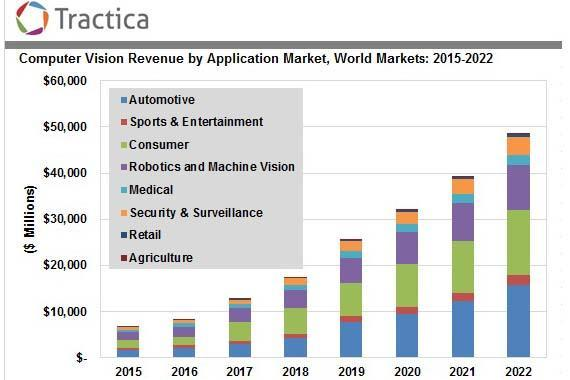
\includegraphics[width=10cm]{cv_forecast_2022}
	\caption{Computer Vision revenues in the last year, and forecast for 2022 (source: \cite{cv_forecast}).}
	\label{fig:1_cv_forecast}
\end{figure}

One of the mostly used approaches is commonly called the \textit{Viola-Jones} detector \cite{violajones}. This algorithm relies on a \textit{rigid body model}, which fits a specific shape. On a grayscale image, this shape can be typically distinguished by means of the pixel intensity levels. A spatial filters called \textit{Haar features} (\autoref{fig:1_haarfeats}) are introduced: these are used across the image looking for the intensity pattern for each mask, which should resemble a part of the rigid body. As this presents a weak decision by itself, several filters (previously chosen in a training process) are combined on a \textit{boosted cascade}. A person is detected if the weighted combination of several filters are triggered inside a certain area, which is decided to potentially contain a person \cite{diapos_cv_clasif}.

\begin{figure}[h]
	\centering
	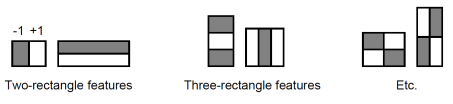
\includegraphics[width=0.7\linewidth]{haar_feats}
	\caption{Haar features: some examples \cite{diapos_cv_clasif}.}
	\label{fig:1_haarfeats}
\end{figure}

\begin{figure}[h]
	\centering
	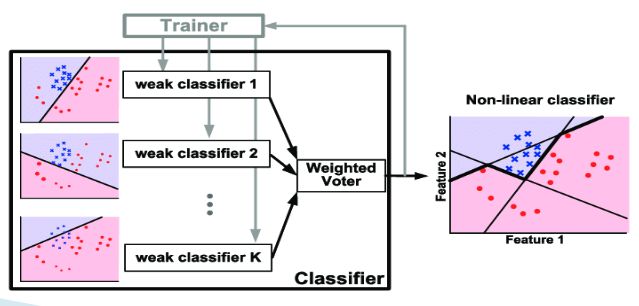
\includegraphics[width=0.7\linewidth]{boosted_cascade}
	\caption{Boosted weak classifiers \cite{diapos_cv_clasif}.}
	\label{fig:1_violajones_boost}
\end{figure}

Although this system was originally developed to detect faces, the rigid body model allows a generalization powerful enough to extend this to another object classes, \textit{person} among these. The open-source standard image processing library, OpenCV, includes pre-trained models\footnote{\url{https://github.com/opencv/opencv/blob/master/data/haarcascades}}, which can be directly used in their Viola-Jones implementation. Scale invariance can be achieved evaluating the image at multiple scales on runtime.


Another common approach nowadays for person detection is based on HoG (\textit{Histograms of Gradients}) \cite{hog_detection}. This method computes local features by means of the intensity gradients across the image, and quantizes them using their angle (creating a histogram for the oriented gradients for that pixel), as it can be seen on \autoref{fig:1_hog_sift}.\\


\begin{figure}[h]
	\centering
	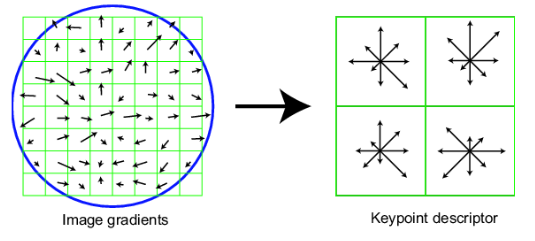
\includegraphics[width=0.7\linewidth]{hog_sift}
	\caption{Example of a HoG, quantized to 8 directions \cite{diapos_cv_features}.}
	\label{fig:1_hog_sift}
\end{figure}



These gradients are collected in $64 \times 128$ windows, and treated as features from which a linear SVM (\textit{Support Vector Machine}) is trained in order to classify a region as \textit{person/non-person}. \autoref{fig:1_hog_avg} shows the average gradient patch for a person (the direction of each gradient is not shown). A visual inspection immediately resembles the shape of a person standing up. Thus, this detector will yield the best performance when the person to be detected stands in that specific pose.

\begin{figure}[h]
	\centering
	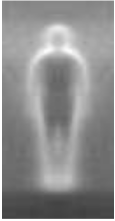
\includegraphics[width=3cm]{hog_avg}
	\caption{Average gradient for person detection on \cite{hog_detection}.}
	\label{fig:1_hog_avg}
\end{figure}

These methods, among several more approaches, have been the state-of-the-art techniques: the cornerstone are the image gradients, which can be computed with a high efficiency and present decent performance. However, their main drawback is the \textit{generalization} capability, as a successful detection is highly dependent on the person pose. However, in the latest advances, the detection frameworks have moved towards the spreading framework: \textit{deep learning}, especially the most salient tools on image processing: CNNs (\textit{convolutional neural networks}). The first steps on this field \cite{rcnn} required for a previous step on the image called \textit{region proposal}. This step is devoted to find potential regions on the image to contain an object. This way, the challenge was to label these region according to the objects contained inside, reducing the problem to a classification task. However, the process to find these undetermined regions and iterate over them makes the process too slow for real-time requirements, which are explicitly contained in our objectives. Care has been put in posterior works \cite{fastrcnn} \cite{spp} to reduce this computation time. However, this reduction in time brings about a reduction in precision as well.\\


On the other hand, one of the most remarkable architectures is SSD (\textit{Single-Shot Multibox Detector}) \cite{ssd}. The main benefit from this architecture is the fact that it embeds all the required computations in a single neural network, reducing the complexity compared to other approaches requiring external region proposals, as it was depicted above. This greatly reduces the computational time when the network has to evaluate an image. As it was depicted in \cite{tfg}, the architecture is split into stages:\\

% ============================================================================

\begin{description}
	
	\item[Reshape] the posterior stages evaluate the image on a fixed tensor size of $n \times 300 \times 300 \times 3$ (being $n$ the size of the input batch). Other image sizes might be used, however this one offers a good trade-off between score and computational load.
	
	\item [Base network] this first group of layers are reused from a typical image classification model, such as VGG-16 \cite{vgg16}. The first layer from this architecture are utilized in this design, truncated before the first classification layer. This way, the network can leverage the \textit{feature maps} from the classification network, in order to find objects inside the input image. At the output of this network, several convolutional layers are appended, decreasing in size. This has the objective of predict detections at multiple scales. One thing to mention at this point is that the base network can be a different one rather than VGG-16, such as a MobileNet \cite{mobilenet}, which is highly optimized for running on low specifications devices. This is interesting as our embedded system will be limited in computing power, thus it will be revisited in future sections.
	
	\item[Box predictors] later, for each extracted set, a dedicated operation is performed, generating a small set (typically 3 or 4) fixed-size \textit{anchors}, with varying aspect ratios for each cell on a grid over the activation map (\autoref{fig:5_ssd_generated_boxes}). As these maps have different sizes, this aims to detect  objects in different scales. The anchors are then convolved with small filters (one per depth channel), which output \emph{softmaxed confidence values for each known class}, and \emph{offsets/adjustments for the generated bounding box}. So, for each detected object (on that scale), we know the score for each class and its estimated position inside the feature map (hence, in the image as well).
	
	\item \emph{Postprocessor}: as several detections might be triggered in the same area for different classes and scales, a \textit{Non-Maximum-Supression} operation is performed at the output of the network to retain the boxes with a larger area.
\end{description}
	\begin{figure}[h]
	\centering
	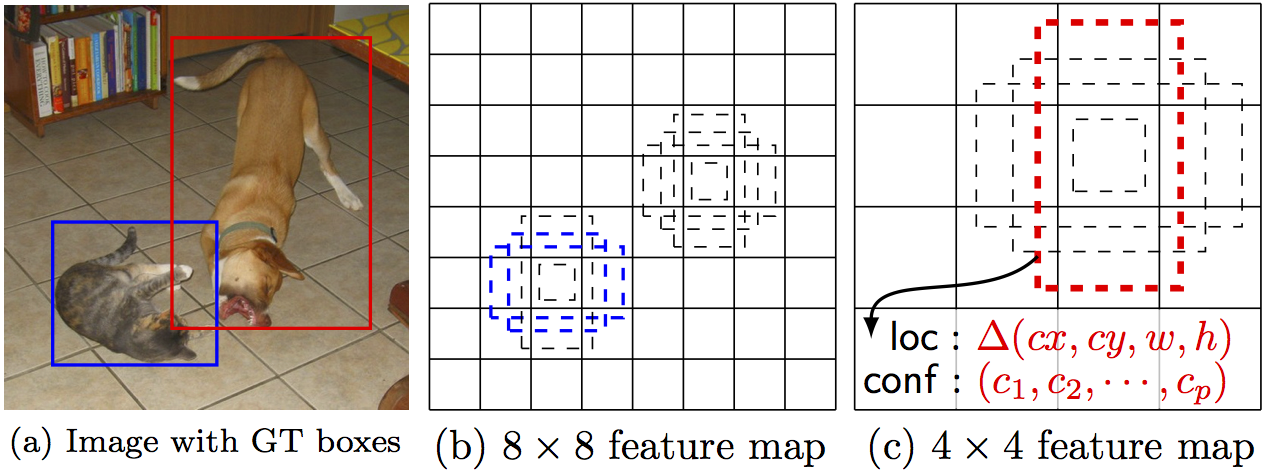
\includegraphics[width=0.7\linewidth]{ssd_generated_boxes}
	\caption{A set of boxes are generated centered on each point of every feature map \cite{ssd}.}
	\label{fig:5_ssd_generated_boxes}
\end{figure}


Another interesting approach on the neural networks field is the YOLO (\textit{You Only Look Once}) system \cite{yolov1}, which has been iteratively revised in two occasions so far \cite{yolov2} \cite{yolov3}.

The latest implementation, YOLOv3 \cite{yolov3} features residual networks \cite{resnets}, which tackle the problem of \textit{vanishing gradients} when the networks become deeper. The stacking of several layers results on gradients diminishing its value up to a point the precision mode of the machine is not able to handle. The gradients are canceled, burdening the training process, as the first layers parameters take a substantially higher time to converge. The residual networks added in this revision of the design add shortcut connections across the layers, centering the backpropagation gradients on 1. As the publication says \cite{yolov3}, the combination of these residual layers and convolutional ones allows to train much deeper architectures, capable of yielding a higher generalization. As in the SSD detectors, the YOLO architecture performs multi-scale detections, using 3 scales for splitting the feature maps into cell grids. On each of these cells, 3 anchor bounding boxes are fit. These anchors are selected by running the k-means algorithm on the COCO datasets selecting 9 clusters (3 anchor shapes $\times$ 3 scales). This aims to a better generalization as well, as in the R-CNN \cite{rcnn} and the SSD \cite{ssd} the anchor shapes are hand-picked.\\

For each (anchor, cell, scale) combination, this network predicts:

\begin{itemize}
	\item The coordinates of the object inside the anchor. Details can be visualized on \autoref{fig:1_yolo_output}.
	
	\item \textit{objectness} score, which is computed by means of a logistic regression in order to determine the probability of overlap with a ground truth bounding box more than any other prior anchor.
	
	\item 80 scores, as the original implementation is trained in the COCO dataset, which contains 80 classes. These classes might be overlapping (e.g. ``woman" and ``person"). Thus, these scores are computed by independent logistic classifiers and are not passed through a \textit{softmax} operation.
\end{itemize}


\begin{figure}[h]
	\centering
	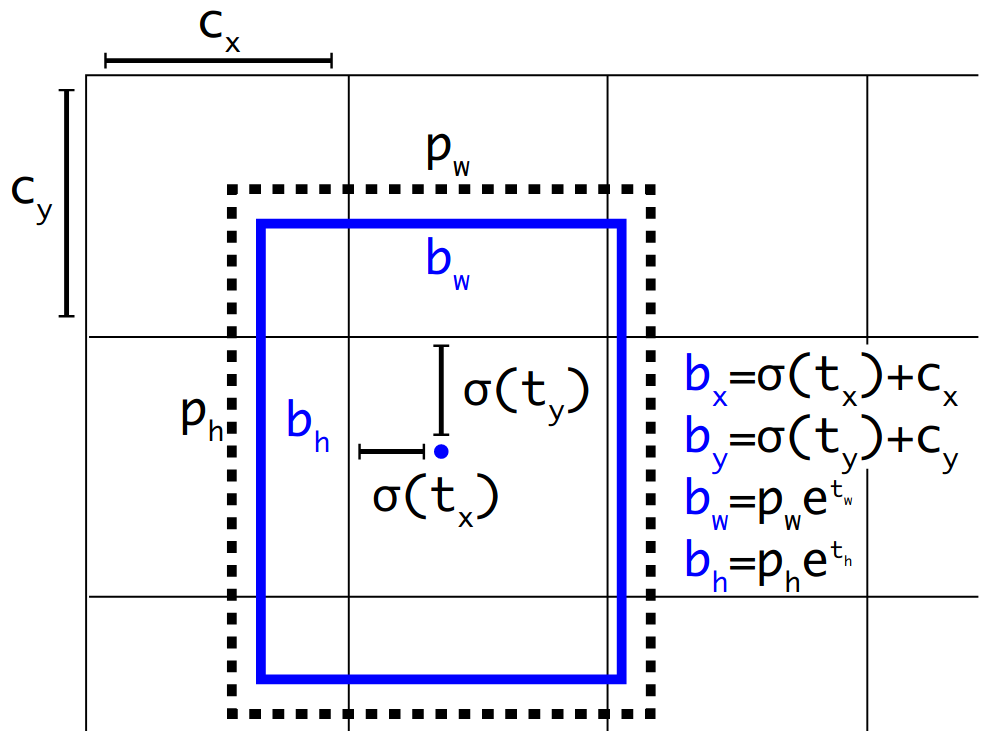
\includegraphics[width=0.5\linewidth]{yolo_outputs}
	\caption{Output on YOLO for each anchor and cell. The dashed line represents the prior anchor, while the blue line represents the detection which corrects that anchor.}
	\label{fig:1_yolo_output}
\end{figure}

\subsection{Person identification}
On a controlled environment, where the only present person is the one to be followed, a person detection system could be enough for following purposes. However, in a normal scenario, there might be several people inside the field of vision of the robot. This problem can be approached by means of adistinguishing feature of the person of interest, provided beforehand. One example is \cite{color_id}, which computes the color distribution of the person of interest, and later compares this distribution with the ones belonging to the different persons using the Bhattacharyya coefficient, which is designed to measure the similarity between the color histograms of the reference person and the detected one. However, this system can be deceived replicating the color distribution of the person of interest: wearing similar clothes helps to reduce the distance between the histogram, leaving a chance to confound another person with the one to follow.\\

A more robust approach is to use the \textit{face} of the person as the distinguishing feature, as its uniqueness makes it a good reference to identify the detected person. Several approaches \cite{dlib_review} extract facial \textit{landmarks} from the morphology of a given face, and use them to classify the face, comparing it against a set of known faces and predicting the identity based on the distance to each known face. Some open-source libraries such as \texttt{dlib} and \texttt{OpenCV} provide the algorithms to perform these processes.\\

\begin{figure}[h]
	\centering
	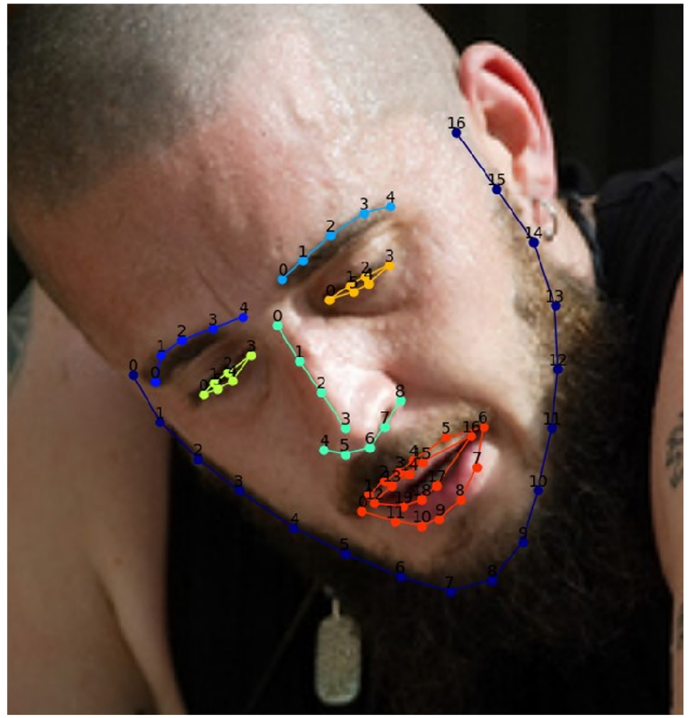
\includegraphics[width=0.6\linewidth]{dlib_landmarks}
	\caption{Facial landmarks are dependent of the face shape and morphology (image from \cite{dlib_review}).}
	\label{fig:1_dlib_landmarks}
\end{figure}


The intuition behind these methods are to \textit{project} the image of the face into a lower dimensional space, which allows to extract significant features from each face. These features have to be consistent for the same face across different pose and lighting conditions (\autoref{fig:1_faces_poses}). An useful transformation when a dimensionality reduction is pursued is PCA (\textit{Principal Component Analysis}), a linear transformation that can be implemented to deal with the face recognition problem \cite{face_pca}.

\begin{figure}[h]
	\centering
	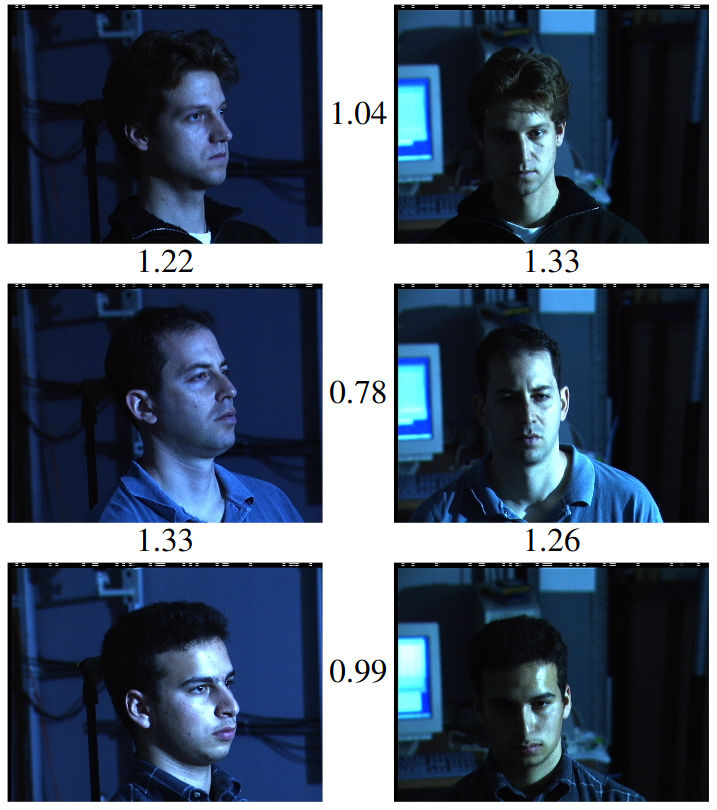
\includegraphics[width=0.5\linewidth]{face_poses}
	\caption{Examples of poses and light conditions across which the face projections are desired to be consistent for the same person (image from \cite{facenet}).}
	\label{fig:1_faces_poses}
\end{figure}


However, once again neural networks can be leveraged in order to achieve this and more: as the PCA is a linear operation, it could be learned by a single layer neural network. Thus, the introduction of deep networks can yield interesting results. The most relevant approach so far uses deep convolutional networks for performing this process \cite{facenet}, implementing an architecture called \textit{FaceNet}, which is partially based on the Inception \cite{inception} module, designed by Google researchers in order to greatly reduce the number of parameters in a neural network. What this network computes is called an \textit{embedding}, a projection of the input face image into a point in a 128-dimensional hypersphere. This allows to translate the identification into linear algebra terms, such as \textit{distance} between two faces, clustering and applying unsupervised algorithms in order to determine the identity of a trivial face, among a collection of known regions. These networks can be trained using a loss function  called \textit{triplet loss}, inspired by the work in \cite{lmnn_loss}. Given a training sample (\textit{anchor}), a \textit{positive} example (same class than the anchor) and a \textit{negative} example (different class than the anchor) are chosen, and the network is tuned to maximize the \textit{anchor-negative} embeddings distance, and minimize at the same time the \textit{anchor-positive} one (\autoref{fig:1_facenet_triplet_loss}).

\begin{figure}[h]
	\centering
	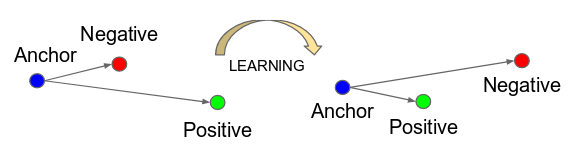
\includegraphics[width=0.7\linewidth]{facenet_triplet_loss}
	\caption{Triplet loss training. It minimizes the distance between an \emph{anchor} (current example) and a \emph{positive}, both of which have the same identity, and maximizes the distance between the \emph{anchor} and a \emph{negative} of a different identity (from \cite{facenet}).}
	\label{fig:1_facenet_triplet_loss}
\end{figure}


One thing to mention about the algorithms described above is that they perform the operations on the image of a face. Thus, a face detection system is required for previously cropping the face of the person to be identified. Once again, a neural approach can be reduced to an \textit{object detection} problem (detecting the class \textit{face}, in this case). One interesting approach using this technique is \textit{faced} \cite{faced}. This is a custom small ensemble of two neural networks, responsible to detect faces and correct the bounding boxes found. The main objective of the system is \textit{speed}, so the main detector architecture is based in YOLO \cite{yolov1}, and the second correction stage raises the precision achieved by the detector.

\begin{figure}[h]
	\centering
	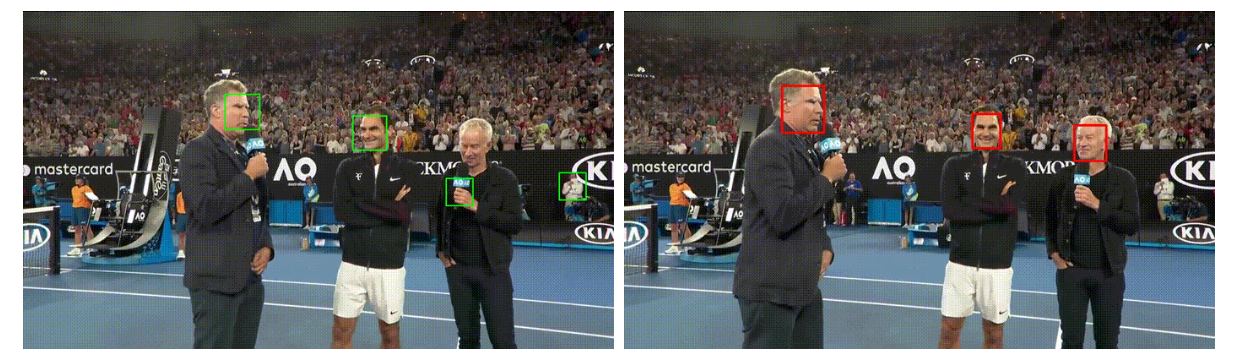
\includegraphics[width=0.8\linewidth]{faced_vs_haar}
	\caption{Classical Haar based face detector \cite{violajones} (left) vs. \textit{faced} (right). Image from \cite{faced}.}
	\label{fig:1_faced_vs_haar}
\end{figure}


%\subsection{Person tracking}

\subsection{Embedded deployment}
One of the requirements of this work is to be integrated in an autonomous system. This imposes a power limitation on the algorithms to be deployed. Generally, the robotic systems are deployed using laptops connected to robots, at it was done in \cite{tfg}.

\begin{figure}[h]
	\centering
	\begin{subfigure}[h]{0.4\linewidth}
		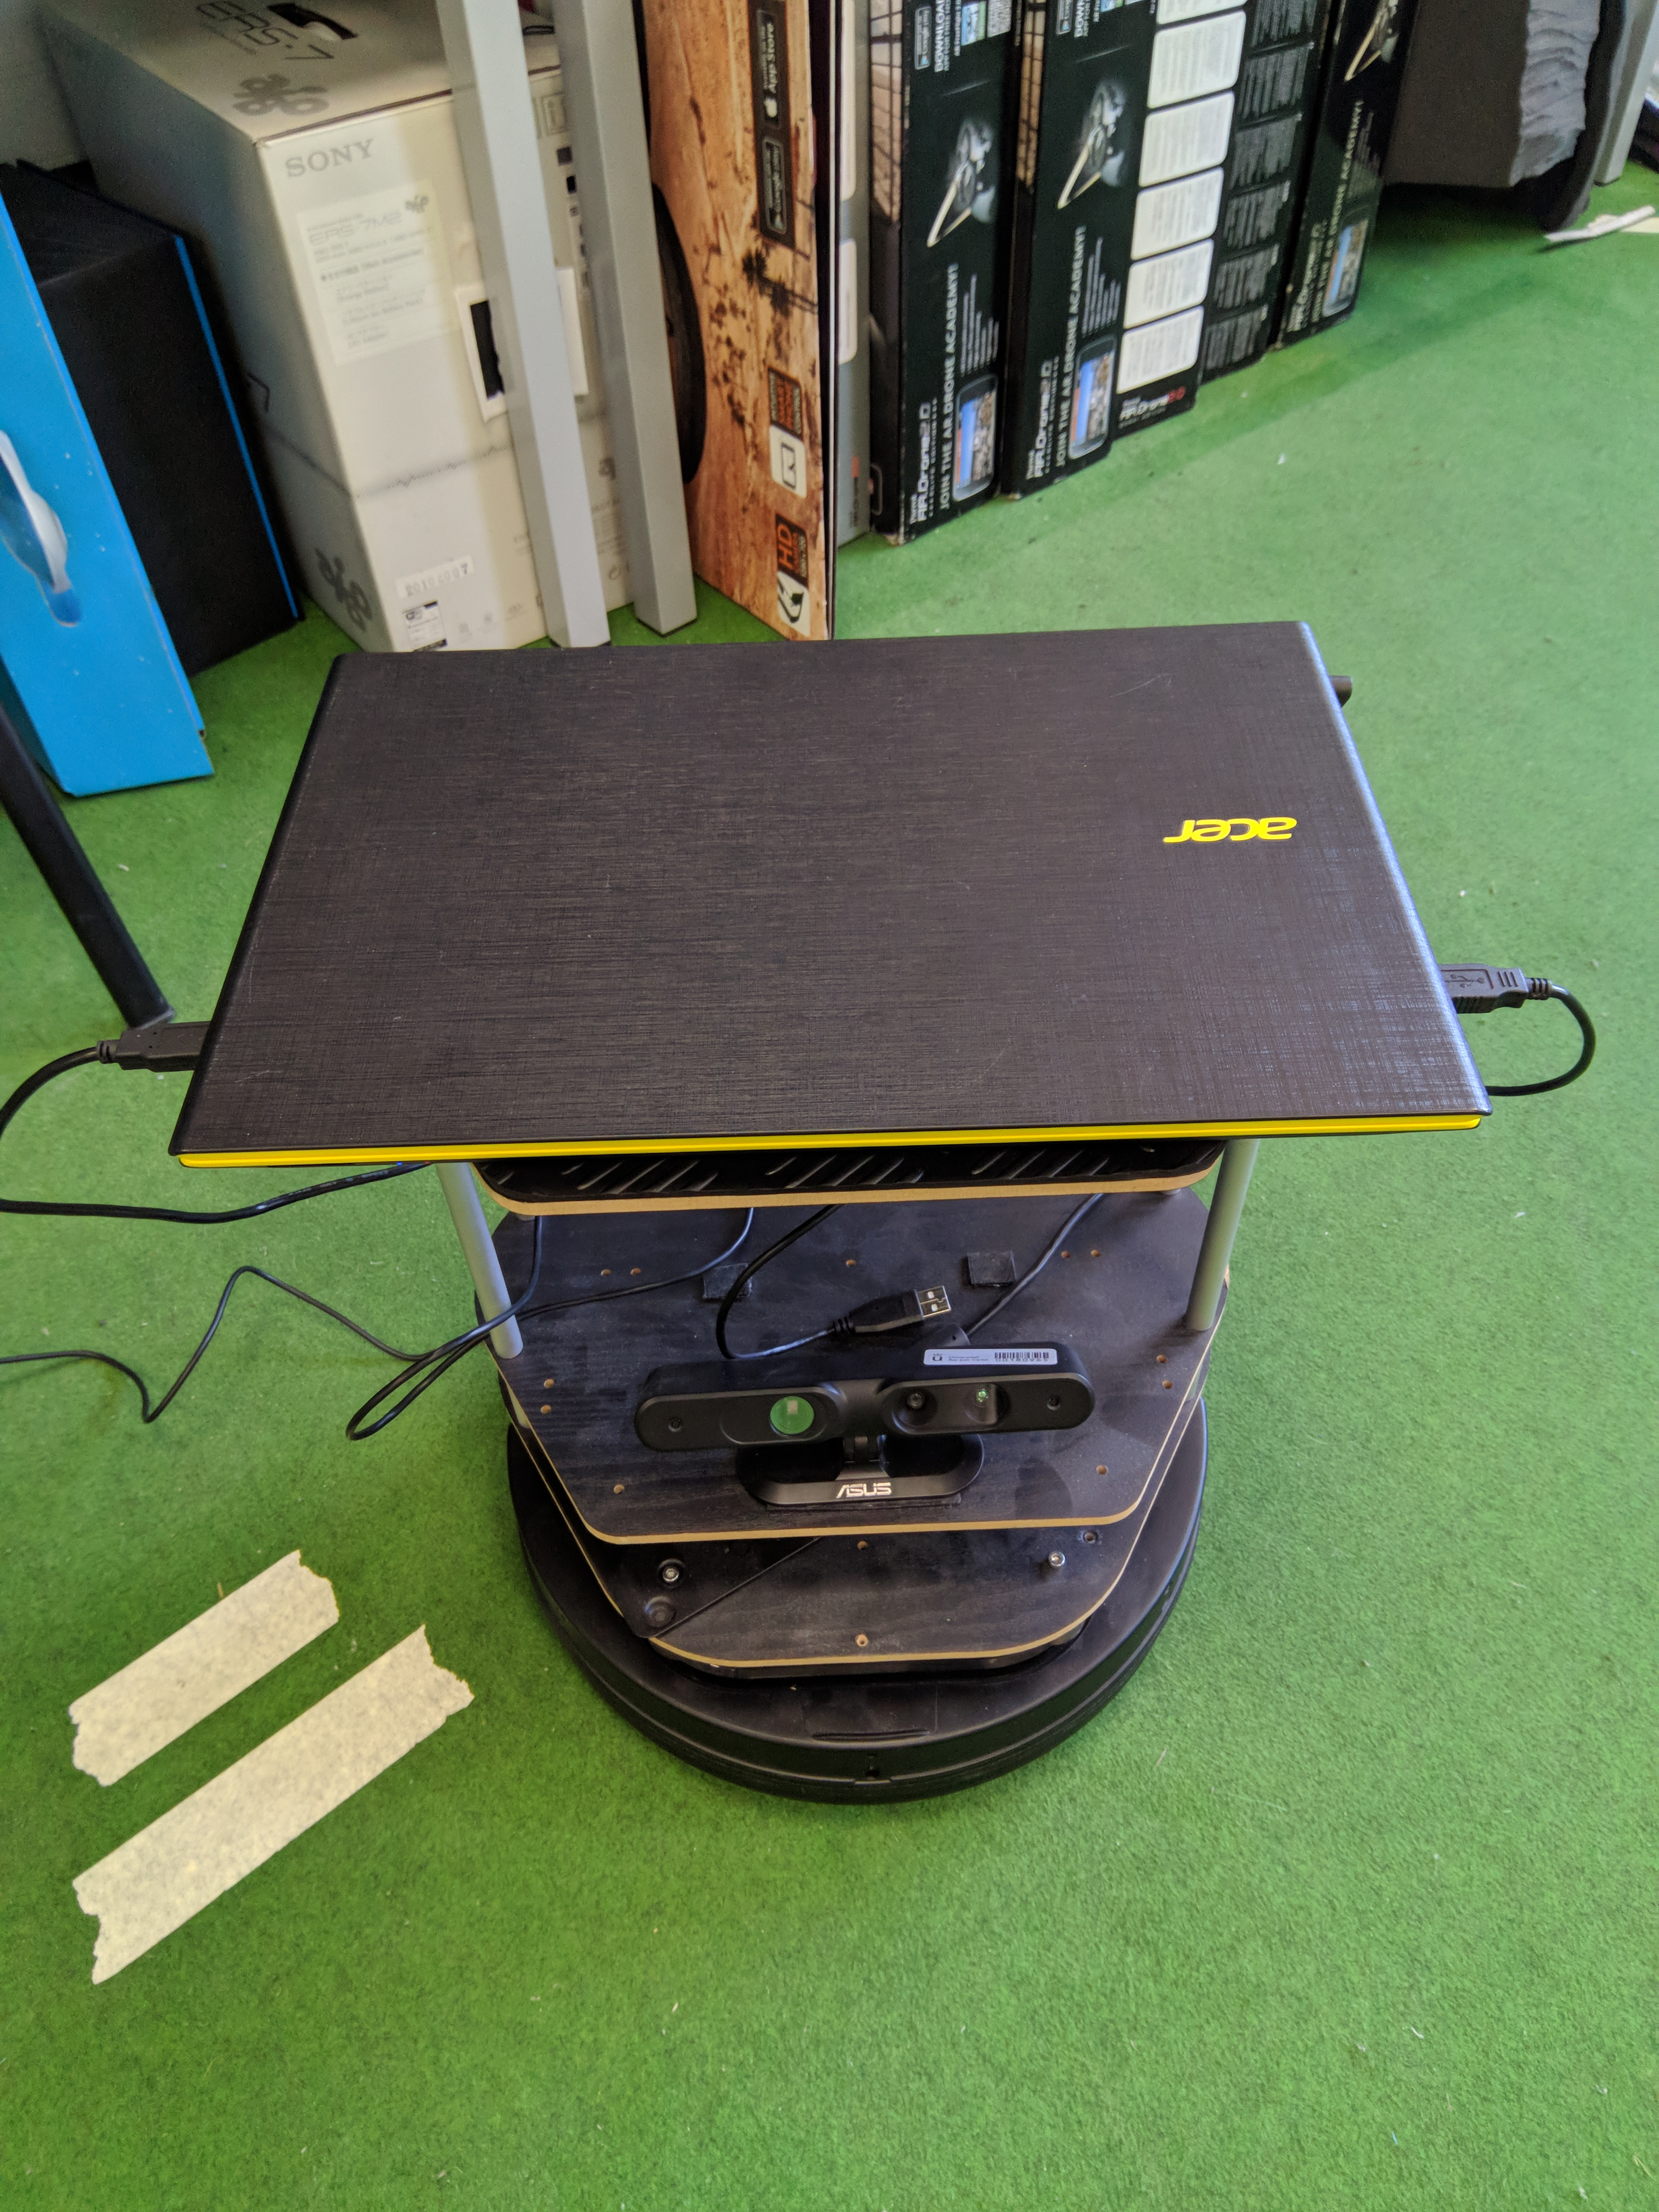
\includegraphics[width=1.9in]{tfg1}
		\caption{Frontal view.}
		\label{fig:3_turtlebot_front}
	\end{subfigure}
	\begin{subfigure}[h]{0.4\linewidth}
		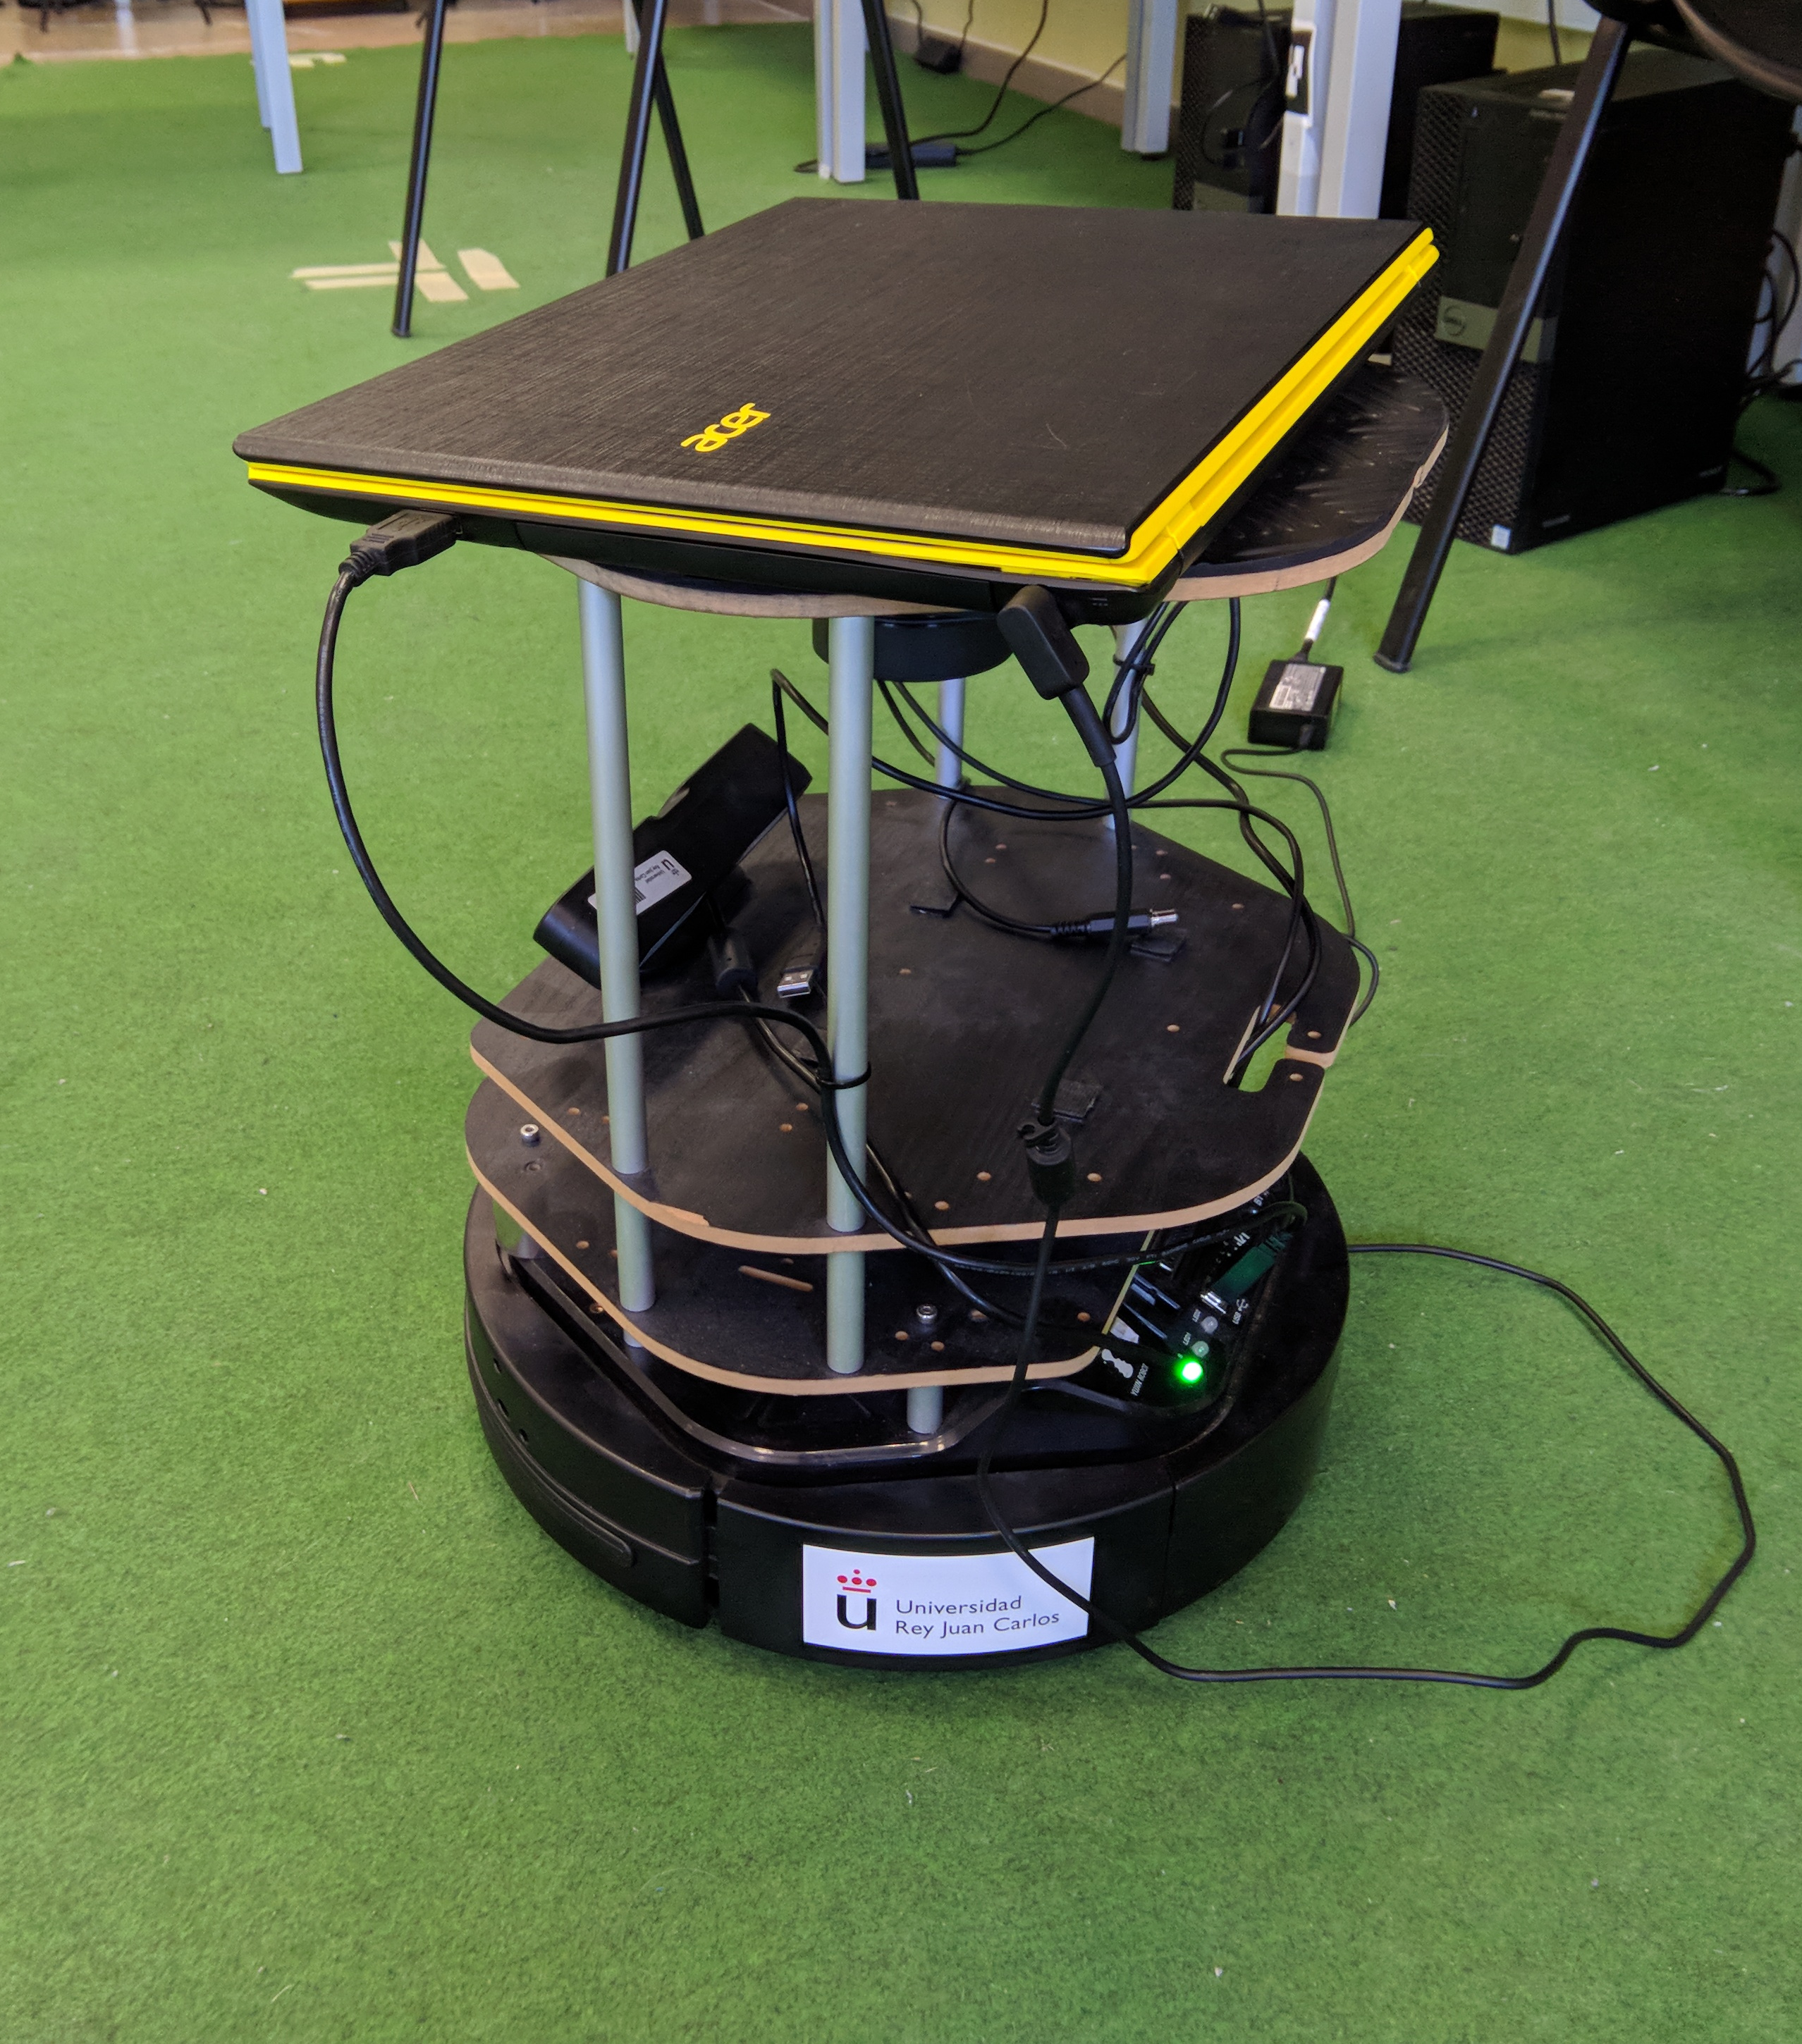
\includegraphics[width=2.2in]{tfg2}
		\caption{Side view.}
		\label{fig:3_turtlebot_side}
	\end{subfigure}
	\caption{Laptop+robot deployment on \cite{tfg}.}
	\label{fig:1_real_tfg}
\end{figure}

Nowadays, the mentioned increase in the interest into the real-time computer vision applications has fostered the development of specific low-power embedded devices to be integrated in mobile systems. The extending usage of devices such as Arduino or Raspberry Pi has led to embedded robotics systems, such as PiBot \cite{pibot} (\autoref{fig:1_pibot}). These robots are useful in the educational scope, as they are capable of running simple vision and navigation algorithms at a low cost.
\begin{figure}[h]
	\centering
	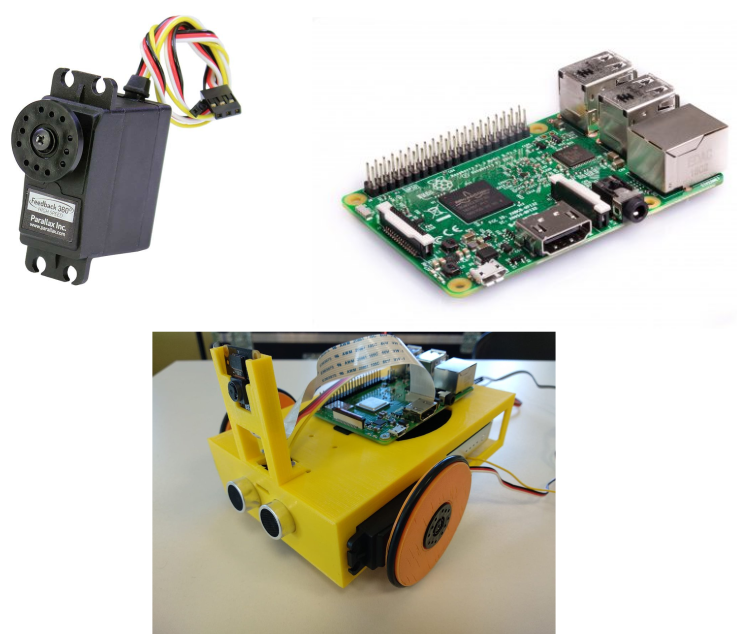
\includegraphics[width=0.5\linewidth]{pibot}
	\caption{PiBot, an open low-cost robotic platform for education (image from \cite{pibot}).}
	\label{fig:1_pibot}
\end{figure}
Unfortunately, the requirements on systems running more complex algorithms, such as neural networks, require of the next tier in power terms, keeping the portability nevertheless. The ideal device could be an ASIC, as the custom design would lead to a very tight optimization of the performance. However, we are aiming to run the algorithms on existing software frameworks, so we aim to general purpose computers instead. The most remarkable advance in this scope are the Jetson devices manufactured by NVIDIA. These development boards are SoM (\textit{System-on-Module}) computers running a tailored version of Linux. The fundamental feature of these systems is that they include a high-performance GPU featuring CUDA, a low-level parallel computation library, as well as several toolkits designed to optimize as much as possible the software implementations for the plethora of possibilities to be designed on this board. As it can be seen in \autoref{fig:1_tx2}, its size and power consumption make of this system a good choice to be included in an autonomous robotic system. 
\begin{figure}[h]
	\begin{subfigure}[h]{0.45\linewidth}
		\centering
		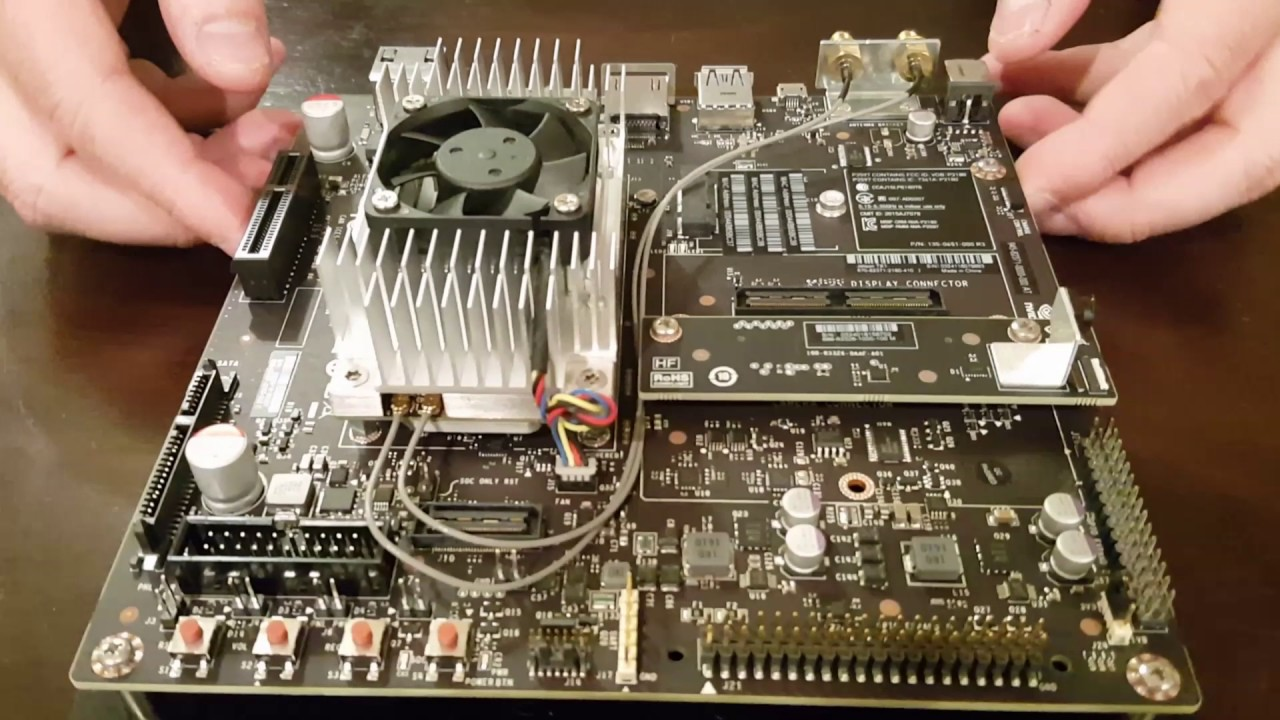
\includegraphics[width=\linewidth]{jetsontx2}

	\end{subfigure}
	\begin{subfigure}[h]{0.45\linewidth}
		\centering
		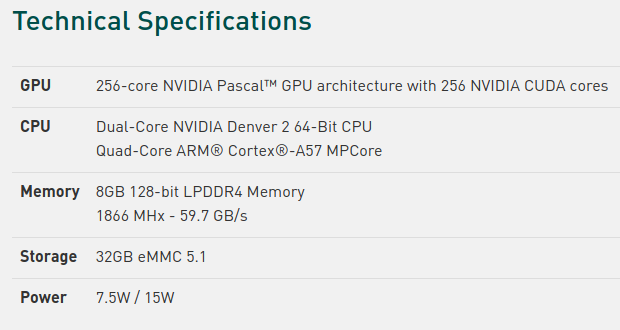
\includegraphics[width=\linewidth]{tx2_specs}
	\end{subfigure}
	\caption{NVIDIA Jetson TX2: an embedded high-performance device including a GPU.}
	\label{fig:1_tx2}
\end{figure}


\subsection{Person following}
Several approaches have been developing pursuing this challenge of \textit{following a person}. Once the perception algorithms are established, the final output of the pipeline has to be a movement command for the robot to move towards the desired point. Mobile  robots can be classified according to their locomotion capabilities. A good summary can be that a robot is \textit{holonomic} if the number of its controllable degrees of freedom is equal to its total degrees of freedom. If the controllable degrees of freedom are lower than the total degrees of freedom, the robot is \textit{non-holonomic}.\\

In the case of a holonomic robot, the navigation process is simplified, as the robot can instantaneously move to a desired target. However, a non-holonomic robot needs to perform maneuvers in order to move towards a point.\\

\section{Objectives}
\label{sec:1_objectives}
	This work has been carried out in order to fulfill certain requirements in a particular person following application:
	
	\begin{enumerate}
		\item Achieve a real-time following behavioral using embedded low-power hardware and a low-complexity educational robot.
		
		\item Build the inference pipeline using exclusively concurrent CNNs (\textit{convolutional neural networks}).
		
		\item Combine a neural system with probabilistic filtering to carry out a robust multimodal tracking of the persons in front of the robot. This will provide the system with extra endurance and robustness against detection losses/occlusions.
	\end{enumerate}
	
These objectives allow to summarize the starting point for the development of this project: the available materials are an educational robot equipped with a battery, an embedded \textit{SoM} and a RGB-D sensor.\\

The result will be an autonomous robot which will follow a specific person, whose face has to be known beforehand (using a \textit{reference face} image).

%\chapter{Materials and Methods}
\label{chap:2_materials_methods}
This chapter is devoted to describe the process followed to develop the system. The development strategy is based in splitting up the functionality into different modules, which have been tackled sequentially. The next sections will cover each one of the modules, and will describe the solution. Finally, the full ensemble will be described and tested.\\


\section{Available materials}
\label{sec:2_materials}
\subsection{Hardware}

As it was depicted in \autoref{sec:1_sota}, typical following approaches work on a personal computer attached to a robot. However, our solution is developed using a devoted SoM: the NVIDIA Jetson TX2 (\autoref{fig:1_tx2}). This system features a high-performance GPU, and low-level optimization engines, which greatly reduce the time required to perform the operations required for deep learning applications, such as tensor convolutions. The low power consumption of this board (15W at full power makes it suitable to be embedded in a portable robot equipped with a battery). One drawback of this system is the scarce storage space. However, this can be immediately solved installing an external storage device using the integrated SATA connector it features. In this project, a 120 GB Kingston SSD (\textit{Solid State Drive}) was used for this purpose, leveraging as well on the high transference throughput this device can achieve. It features a 64-bit ARM processor, and it mounts a fully functional Linux system. As it is equipped with two WiFi antennas, a remote control interface can be easily set using SSH connections.\\

\begin{figure}[h]
	\begin{subfigure}[h]{0.45\linewidth}
		\centering
		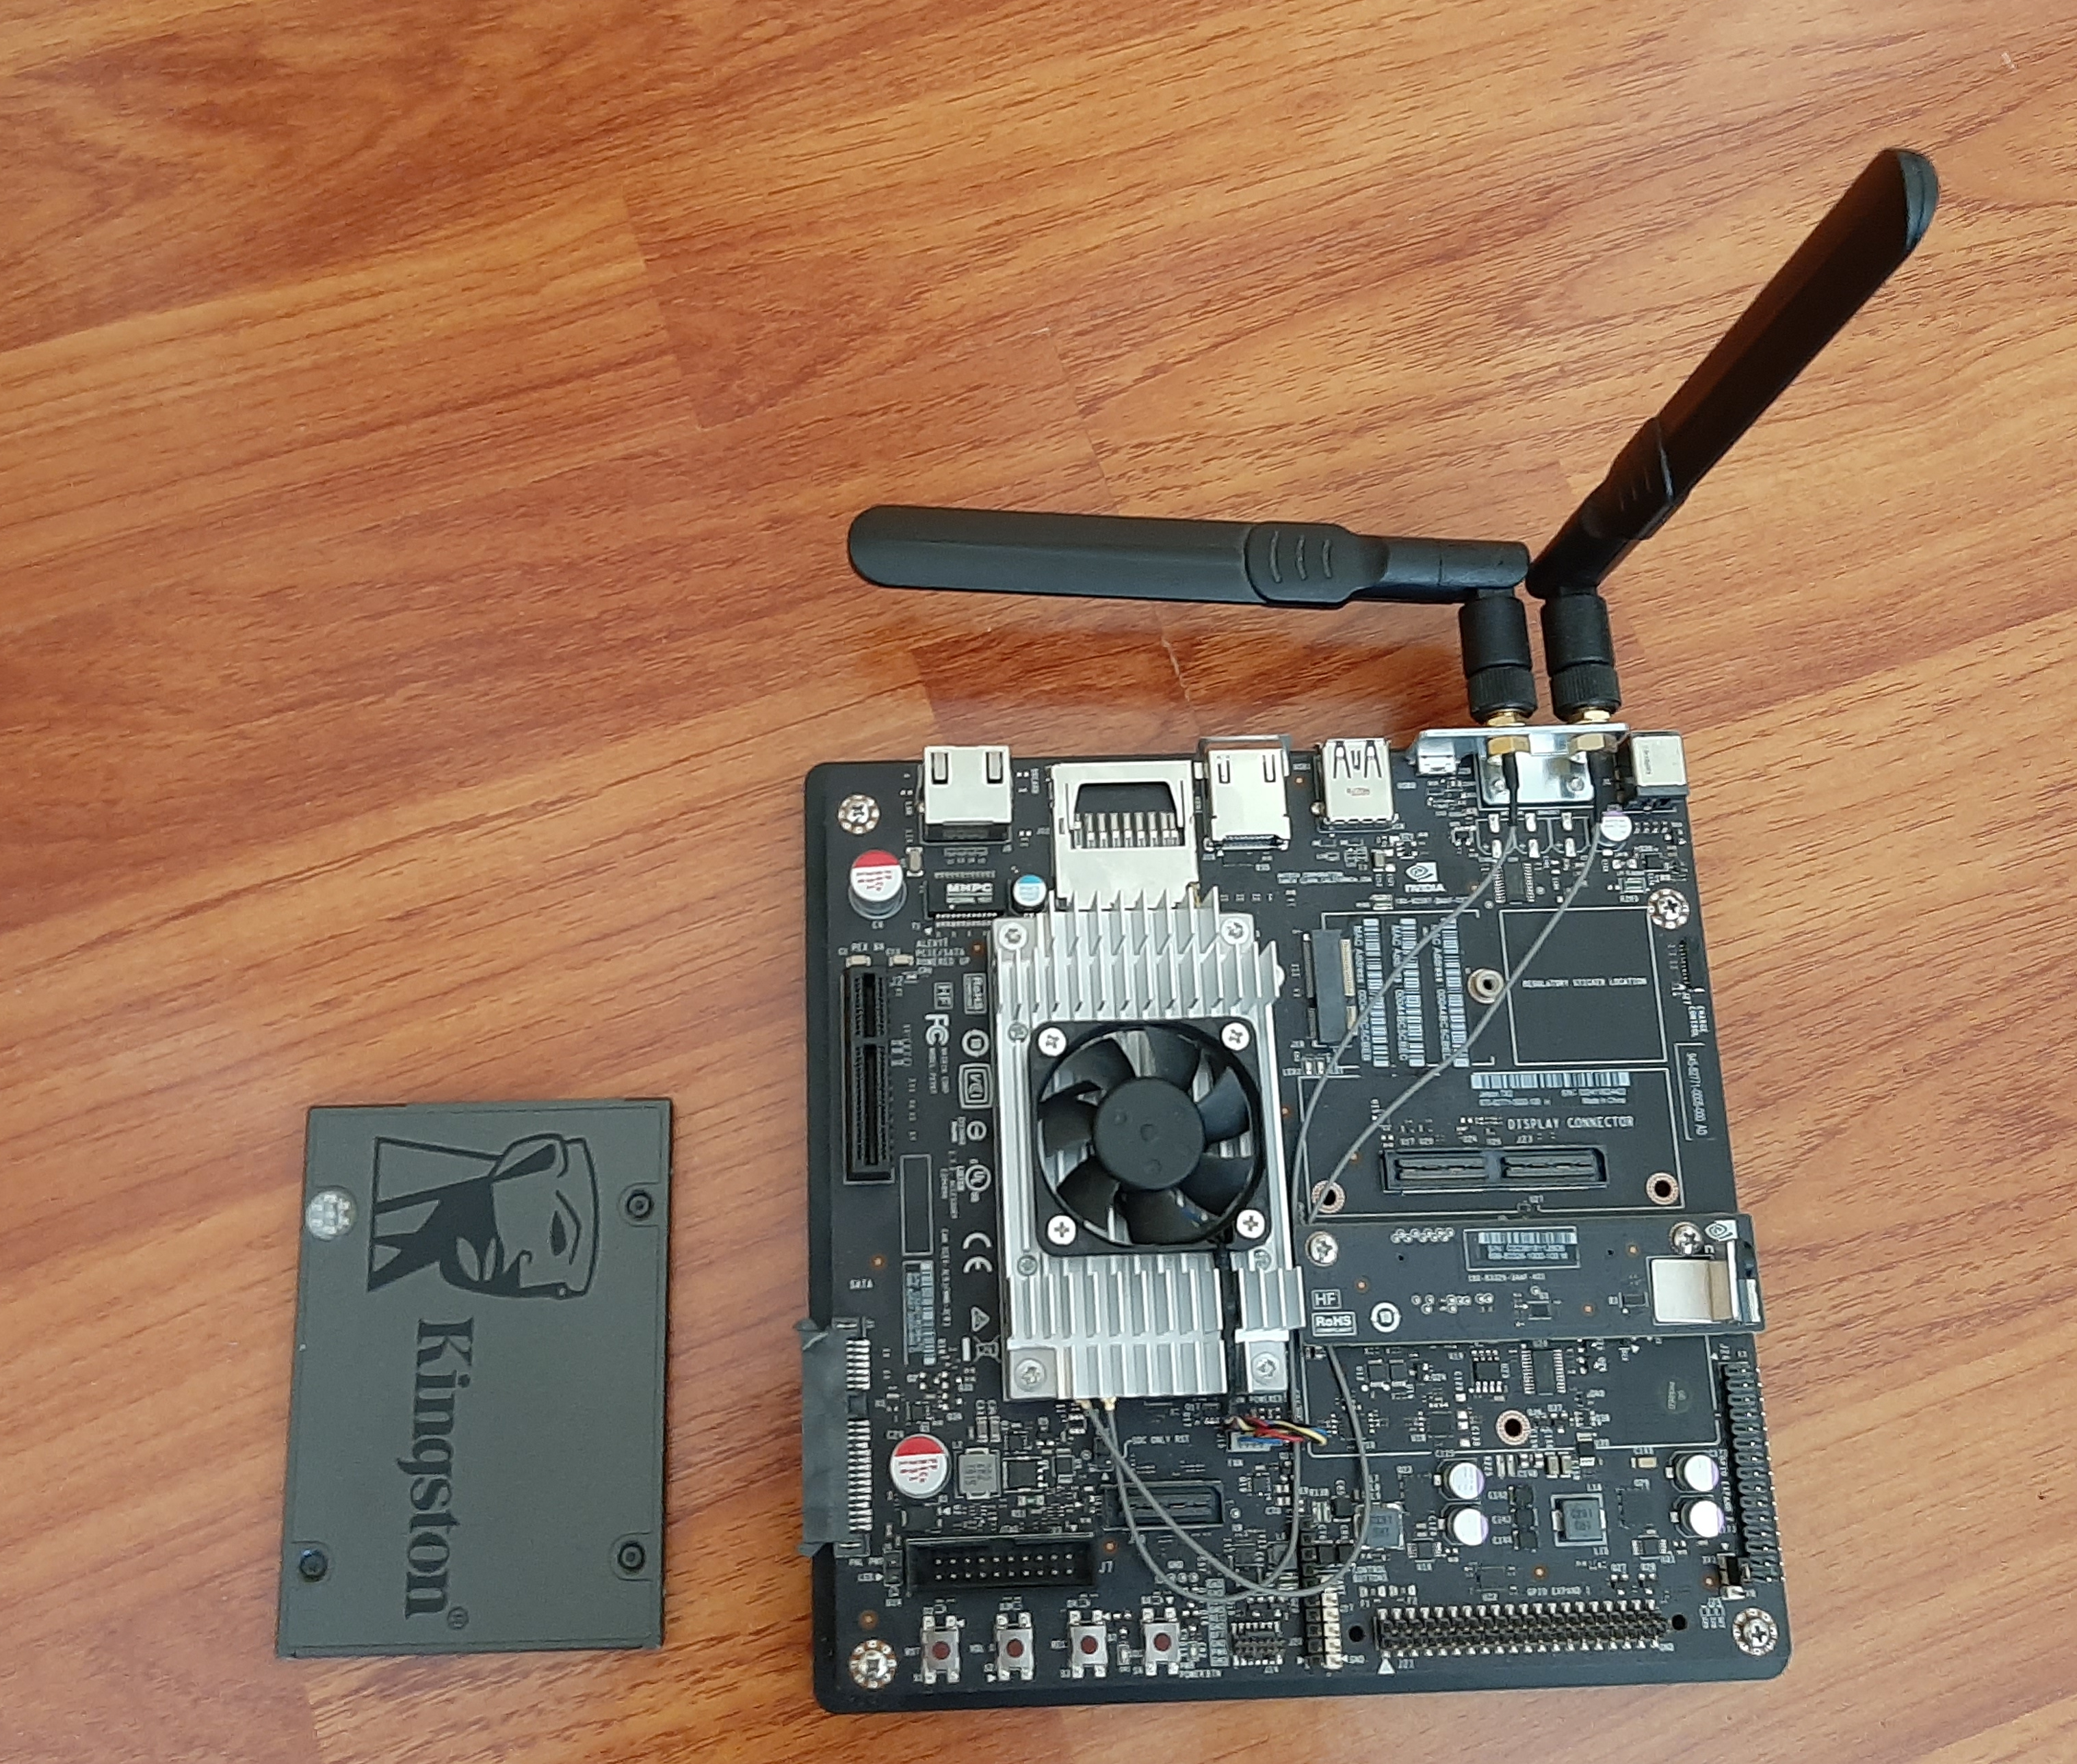
\includegraphics[width=\linewidth]{tx2_nossd}
	\end{subfigure}
	\begin{subfigure}[h]{0.45\linewidth}
		\centering
		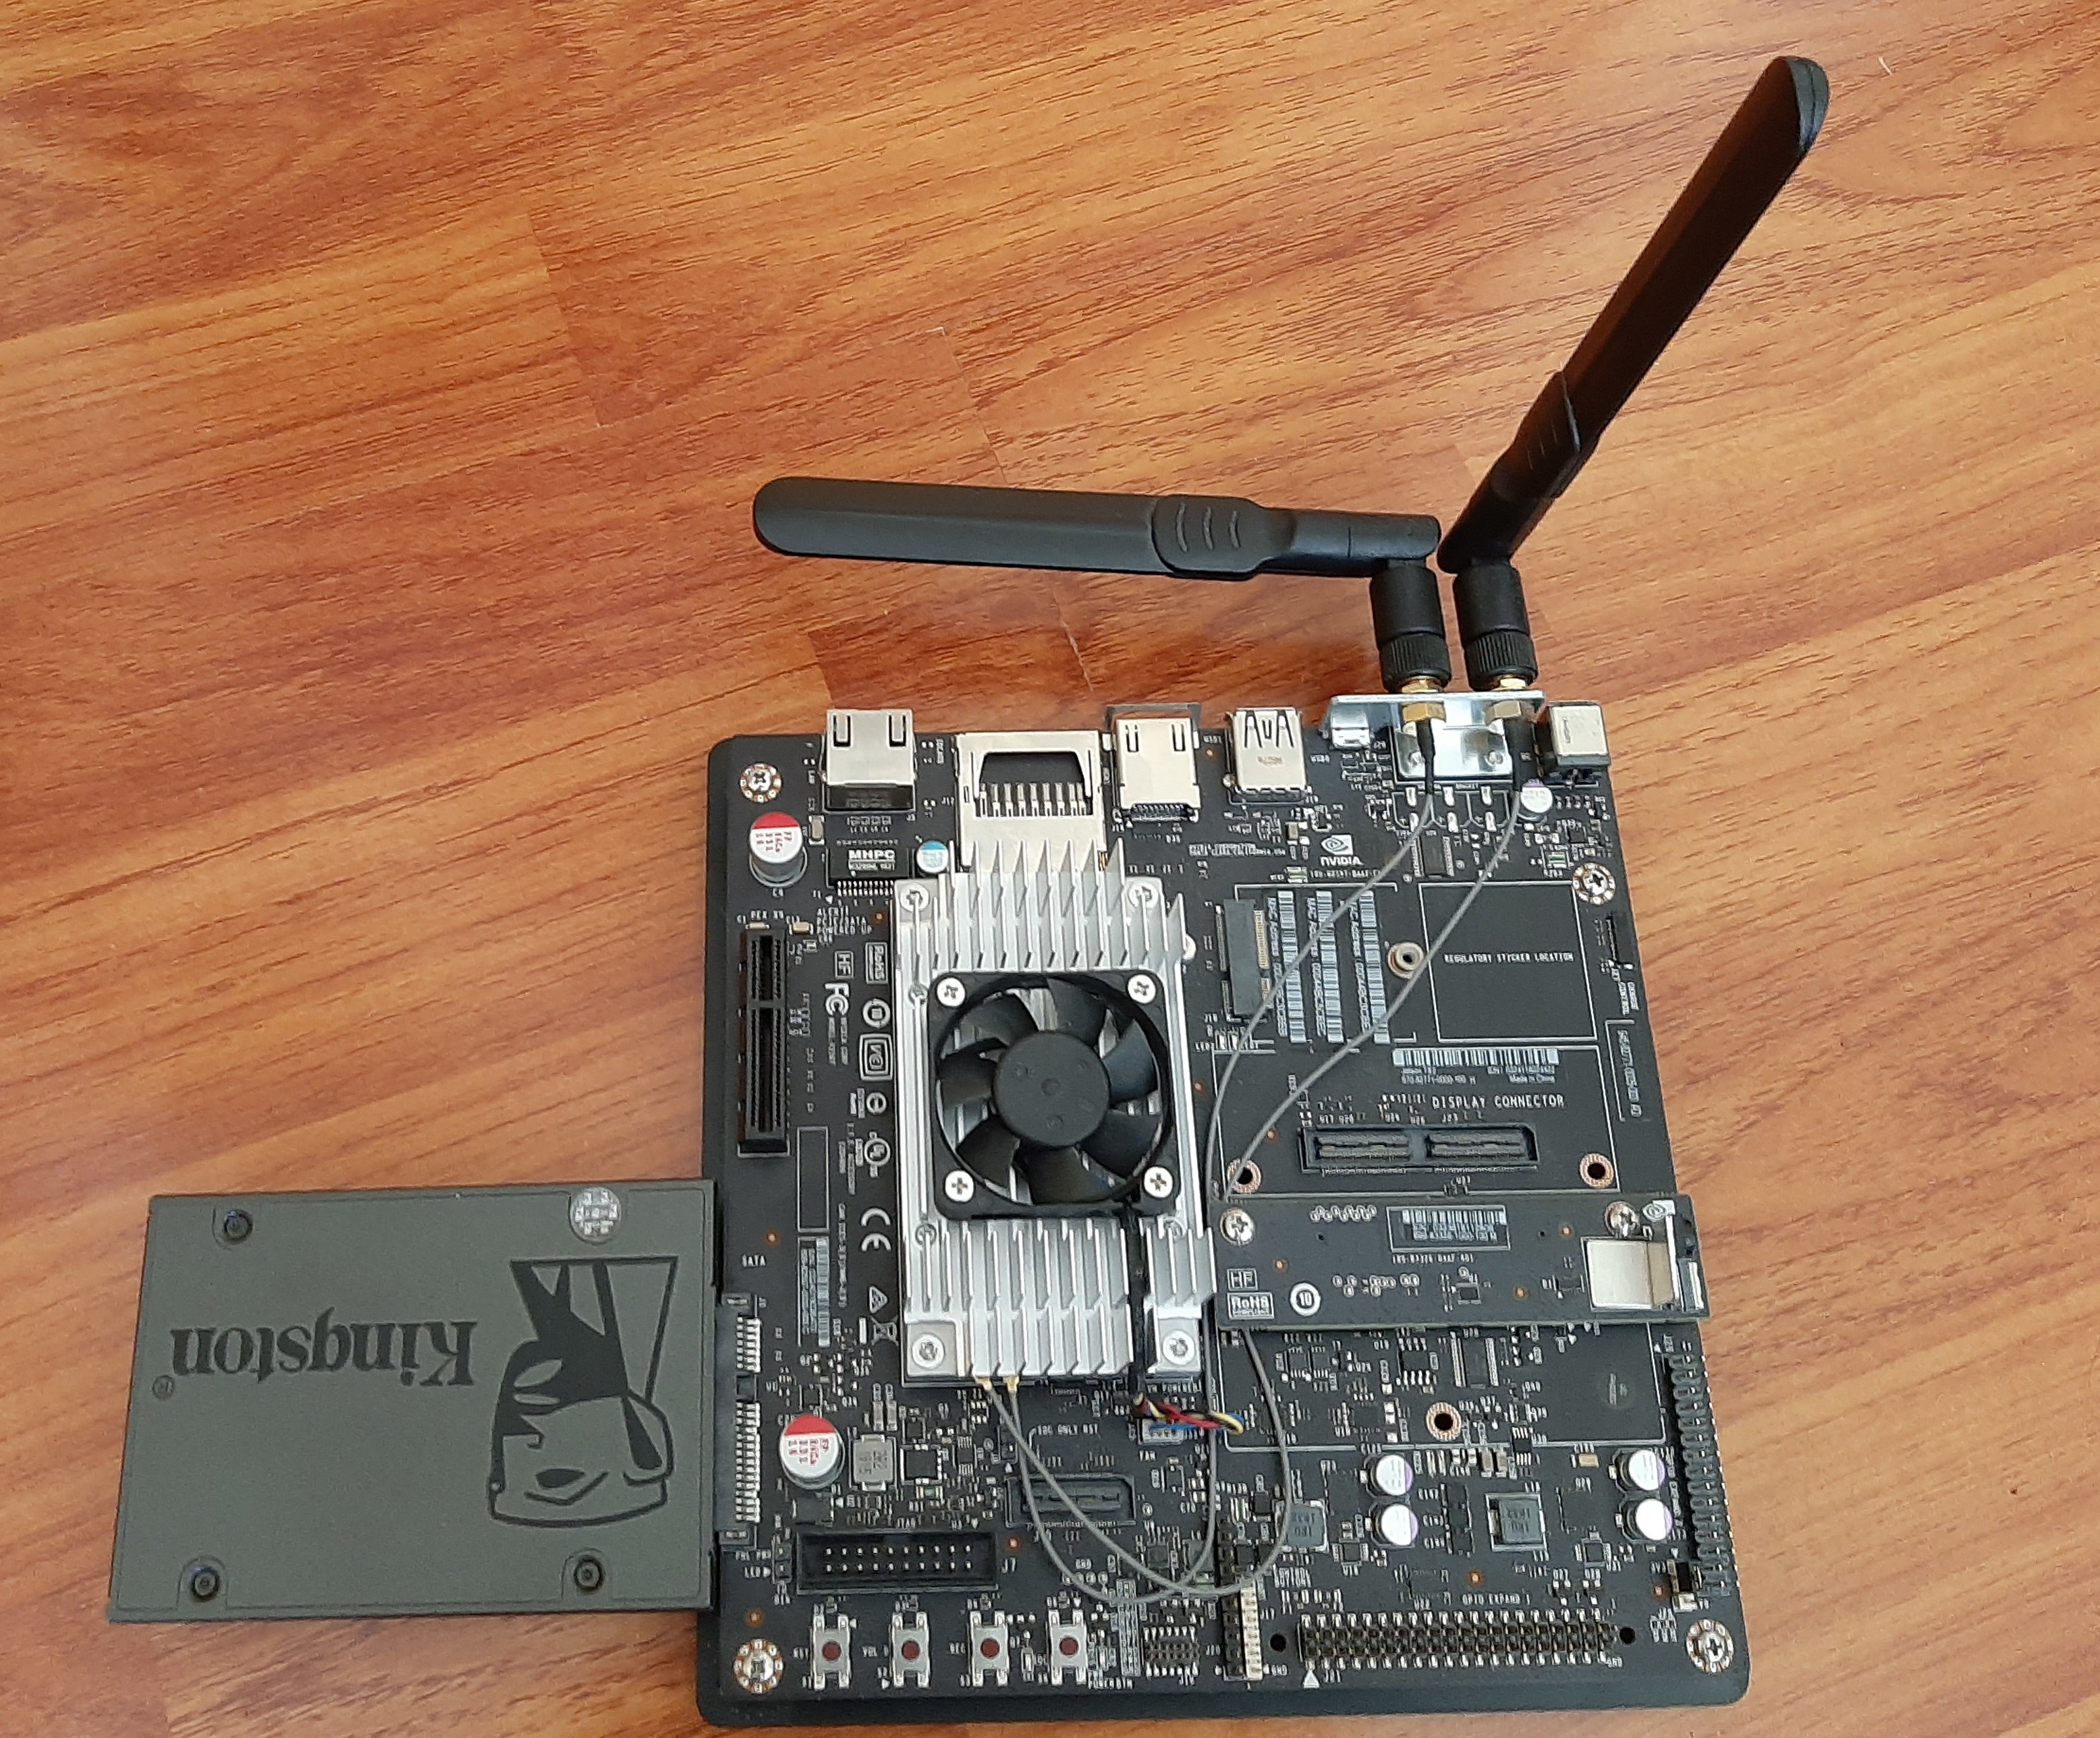
\includegraphics[width=\linewidth]{tx2_ssd}
	\end{subfigure}
	\caption{Resulting system: Jetson TX2 board and the installed SSD drive, plugged into the SATA connector.}
	\label{fig:2_mytx2}
\end{figure}

The vision system used in this work, the ASUS Xtion Pro Live (\autoref{fig:2_xtion}), is a USB device composed by a RGB camera and an IR emitter + sensor system, capable of retrieving depth data for each pixel on the image. This is achieved by emitting a known light pattern (\autoref{fig:2_xtion_pattern}), which reflects in the present surfaces on the scene. These reflections are captured by the IR sensor, inferring the position of the surfaces from the received distribution of the IR pattern.

\begin{figure}[h]
	\centering
	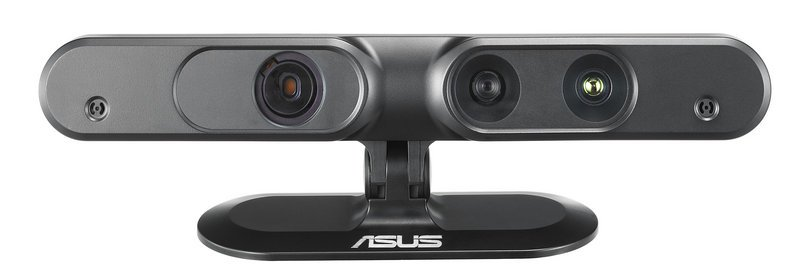
\includegraphics[width=\linewidth]{xtion}
	\caption{ASUS Xtion Pro Live}
	\label{fig:2_xtion}
\end{figure}

\begin{figure}[h]
	\centering
	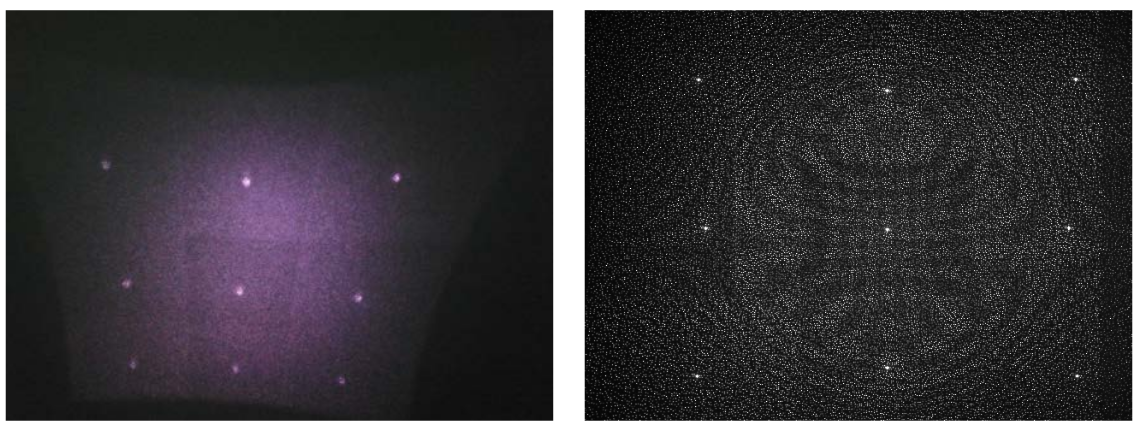
\includegraphics[width=0.9\linewidth]{xtion_pattern}
	\caption{Infrared pattern emitted by the Xtion (images from \cite{rgbd_poses}).}
	\label{fig:2_xtion_pattern}
\end{figure}

The last problem to be tackled by this device is the discrepancy caused by the different points of view of the RGB and depth sensor. However, as the distance between these two sensors is fixed and known, a \textit{registration} process can be carried on inside the device, projecting the depth data into the RGB pixels \cite{diapos_cv_registration}.\\

\begin{figure}[h]
	\centering
	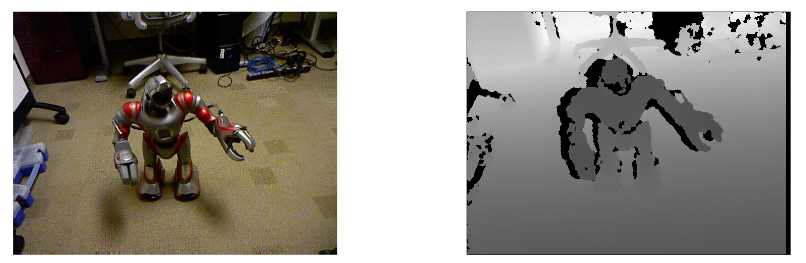
\includegraphics[width=0.9\linewidth]{xtion_discrepancy}
	\caption{Discrepancy between the RGB and depth images (image from \cite{tfg}).}
	\label{fig:2_xtion_discrepancy}
\end{figure}

The systems which implement the described design are called RGB-D sensors, are suitable for robotics, as the yielded result is a point cloud, reflecting the distance from the camera for each pixel in the image. Using this, the device is capable of projecting the 2-dimensional RGB image into the 3D space by means of the depth data (\autoref{fig:2_rviz}).\\

\begin{figure}[h]
	\centering
	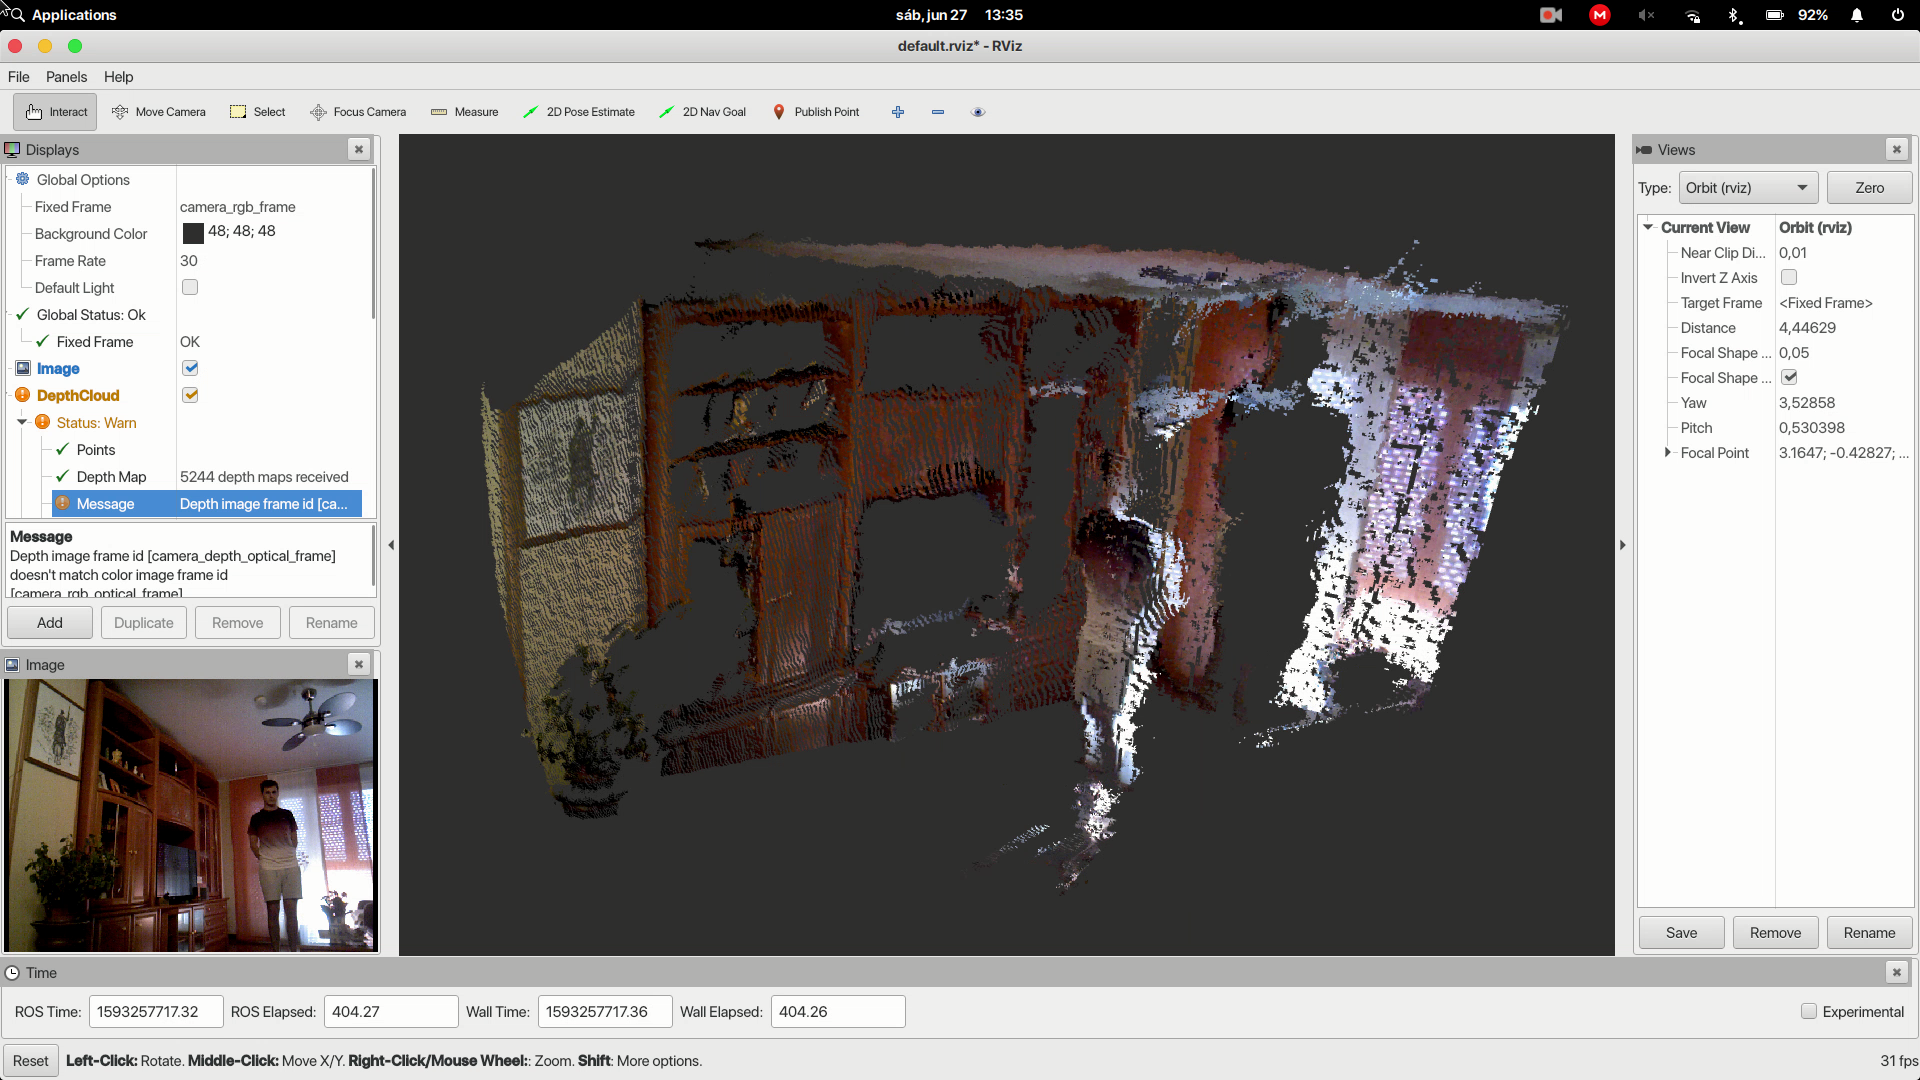
\includegraphics[width=\linewidth]{rviz}
	\caption{Visualization of the RGB image (bottom left) and the resulting point cloud projected into the 3D space (right).}
	\label{fig:2_rviz}
	
\end{figure}

On the other hand, the robot used in this work is the Turtlebot2 educational set. It is based on a Yujinn Robotics Kobuki mobile base (\autoref{fig:2_kobuki}), which is a non-holonomic robot with 2 degrees of freedom: \textit{linear speed} and \textit{angular speed}.\\
\begin{figure}[h]
	\centering
	\begin{subfigure}[h]{0.4\linewidth}
		\centering
		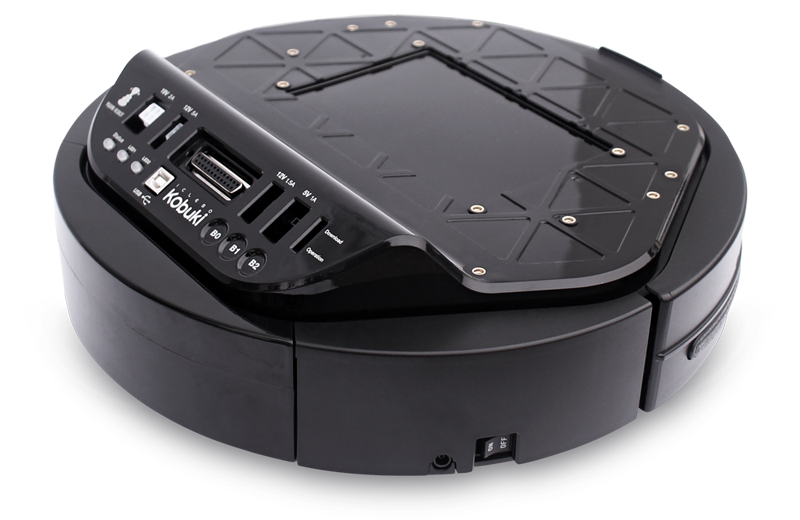
\includegraphics[width=0.9\linewidth]{kobuki}
		\caption{Appearance of the mobile base robot.}
		\label{fig:2_kobuki_appearance}
	\end{subfigure}
\begin{subfigure}[h]{0.5\linewidth}
	\centering
	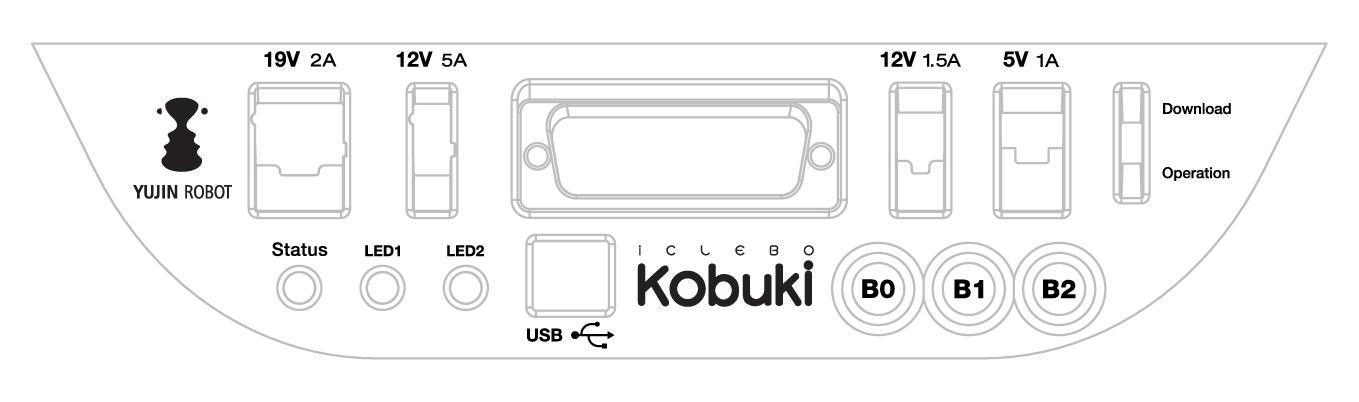
\includegraphics[width=0.9\linewidth]{kobuki_panel}
	\caption{Schematic of the connections panel of the Kobuki.}
	\label{fig:2_kobuki_panel}
\end{subfigure}
\caption{Kobuki mobile base, which carries the rest of the structure.}
\label{fig:2_kobuki}
\end{figure}

In the Turtlebot2 version, the mobile base has an attached structure, carrying the RGB-D sensor and a platform where typically a computer can be placed. This platform is useful to keep the NVIDIA Jetson device. Additionally, as it can be seen in \autoref{fig:2_kobuki_panel}, the Kobuki panel is equipped with a 12V output, yielding up to 1.5A, which in power terms can be translated to a maximum power of 18W. As the TX2 board peak consumption is 15W, this connector is suitable to power the system up, with an additional power margin of 3W. A lookup in the Kobuki user guide \cite{kobuki_manual} allows to find the suitable Molex connector, which can then be attached to two-wire cable and a rounded connector. This provides the NVIDIA Jetson of a 12V DC supply, similar to what it would obtain from a power outlet with a transformer. As the power input is equipped with a DC voltage regulator, it accepts voltages from 5.5V to 19V (table 59 in \cite{tx2_manual}), this is a successful approach to build an \textit{autonomous} system: powering the computing board from the batteries of the robot.\\

The final hardware setup is displayed on \autoref{fig:2_setup}, where the described components are combined to build the autonomous setup capable of running high-complexity person following algorithms.\\

\begin{figure}[h]
	\centering
	\begin{subfigure}[h]{0.45\linewidth}
		\centering
		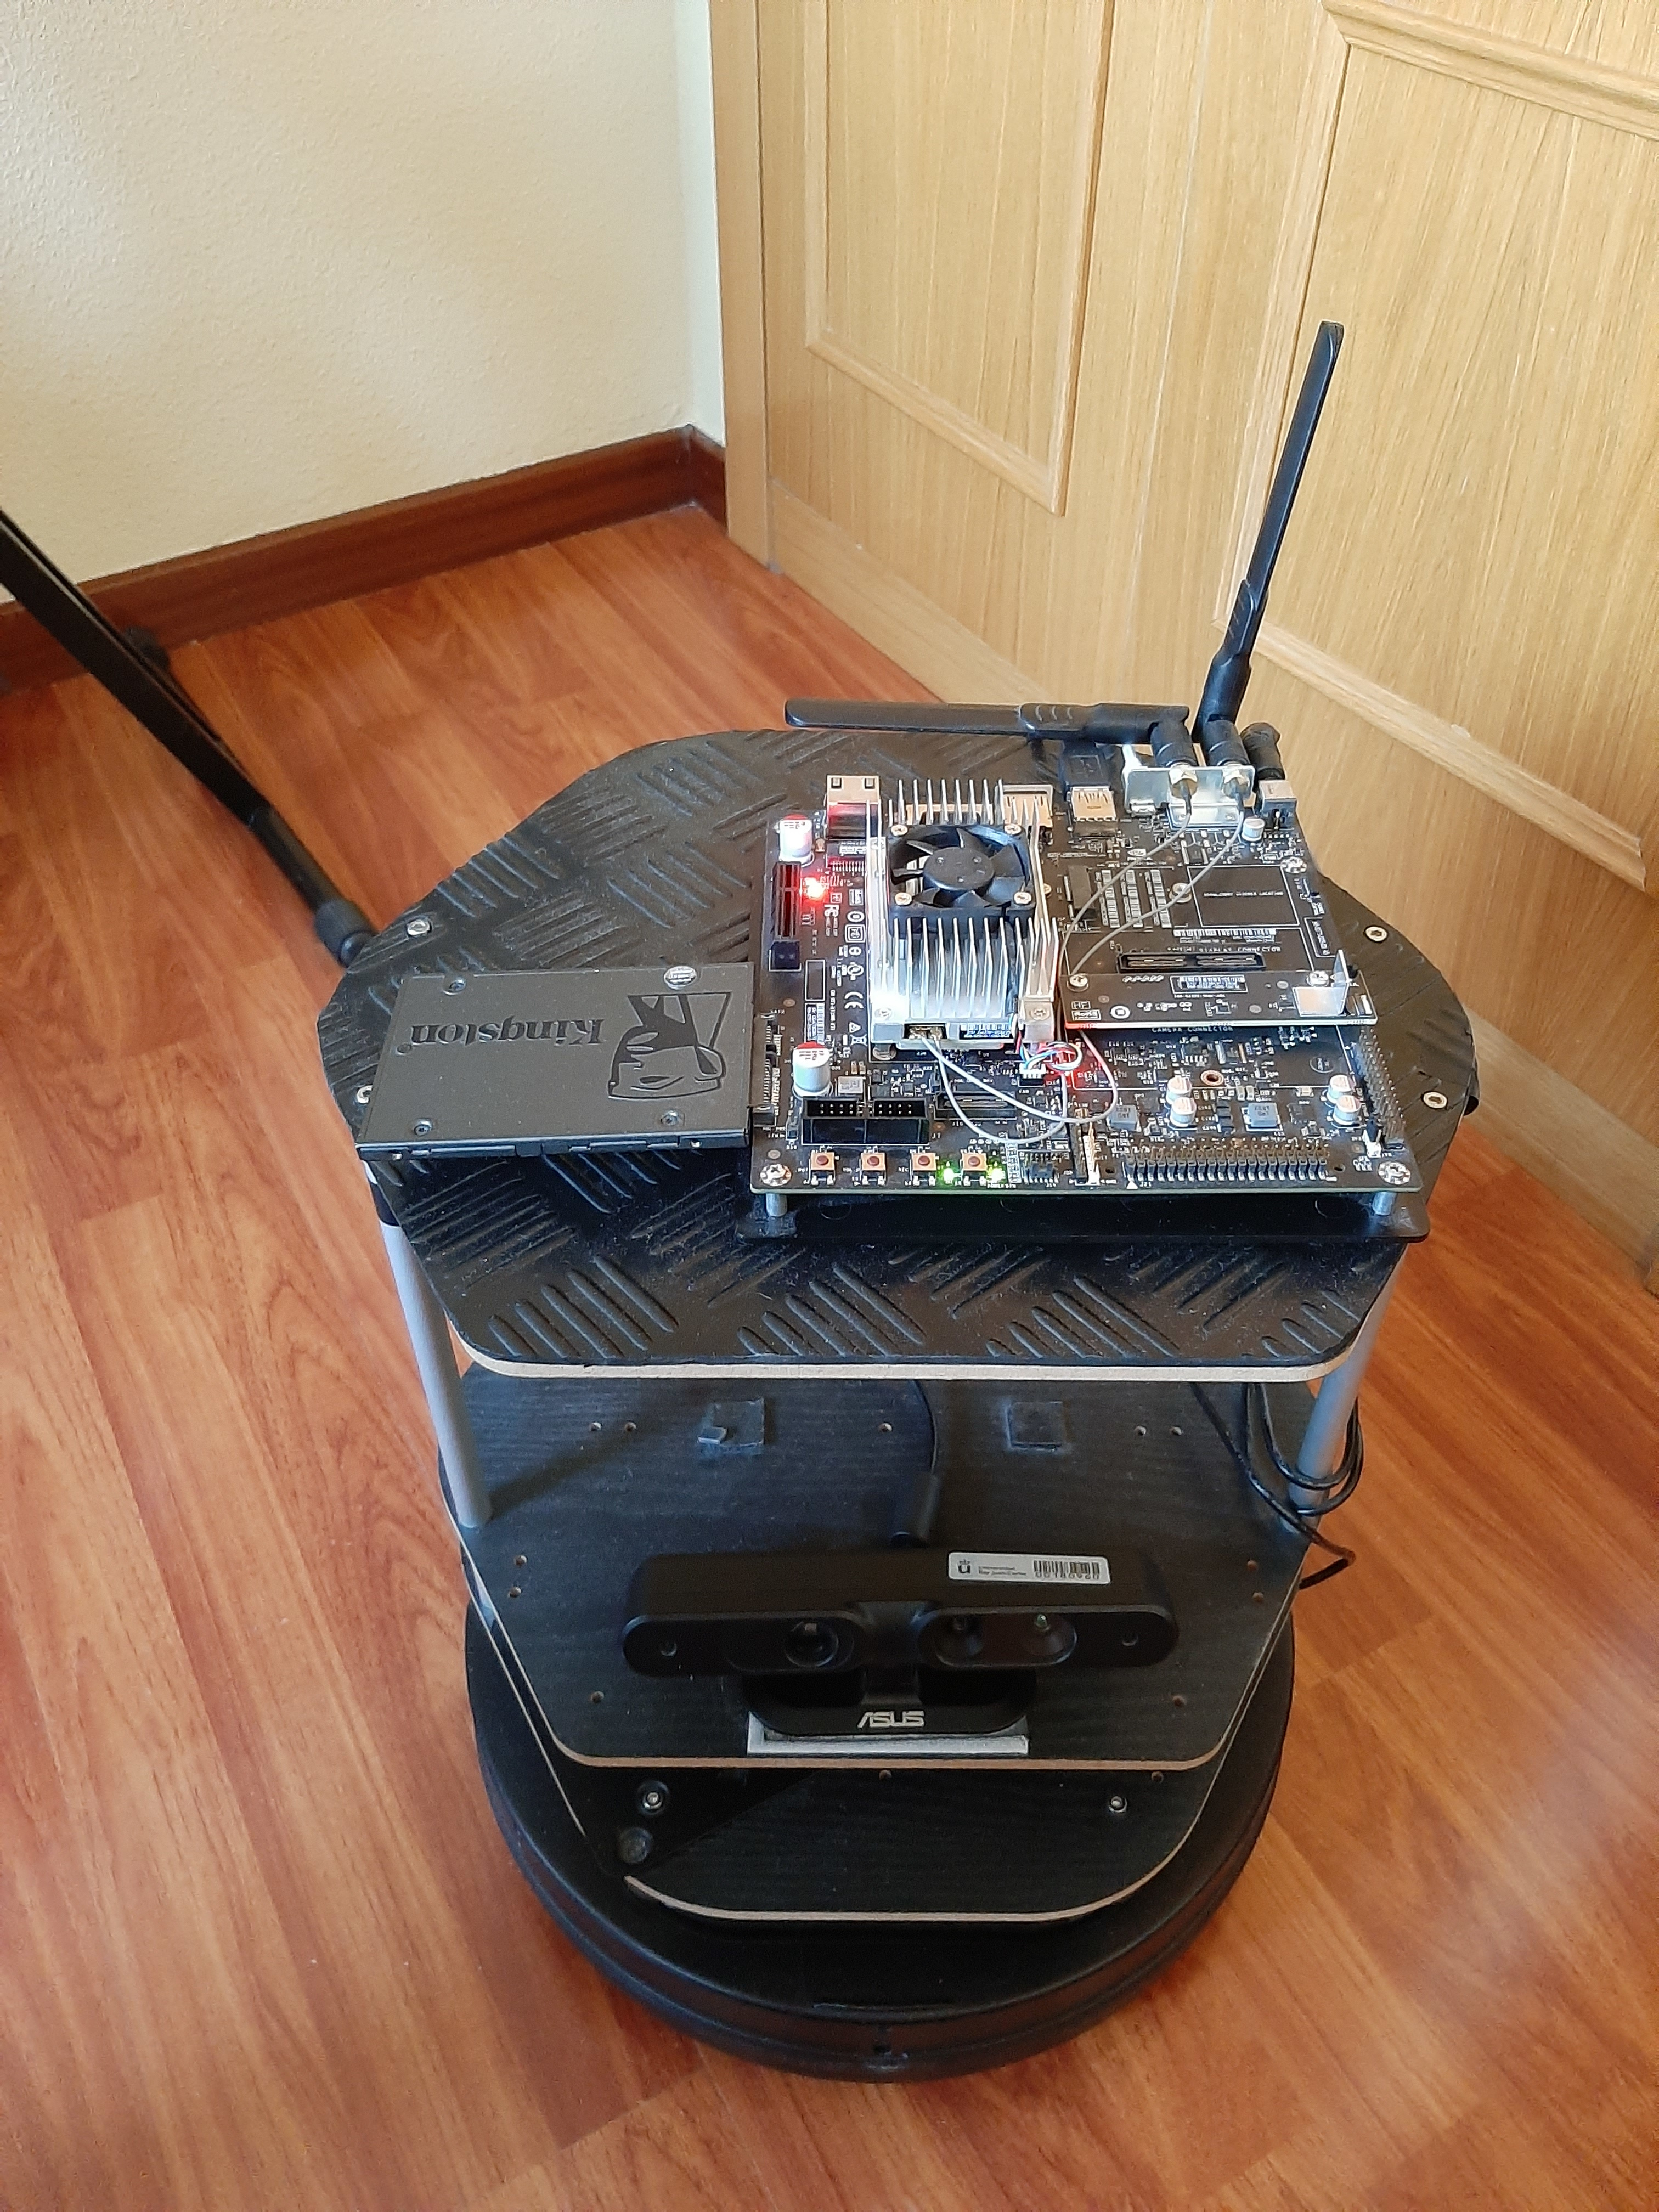
\includegraphics[width=0.9\linewidth]{setup_front}
		\caption{Front view.}
	\end{subfigure}
	\begin{subfigure}[h]{0.45\linewidth}
		\centering
		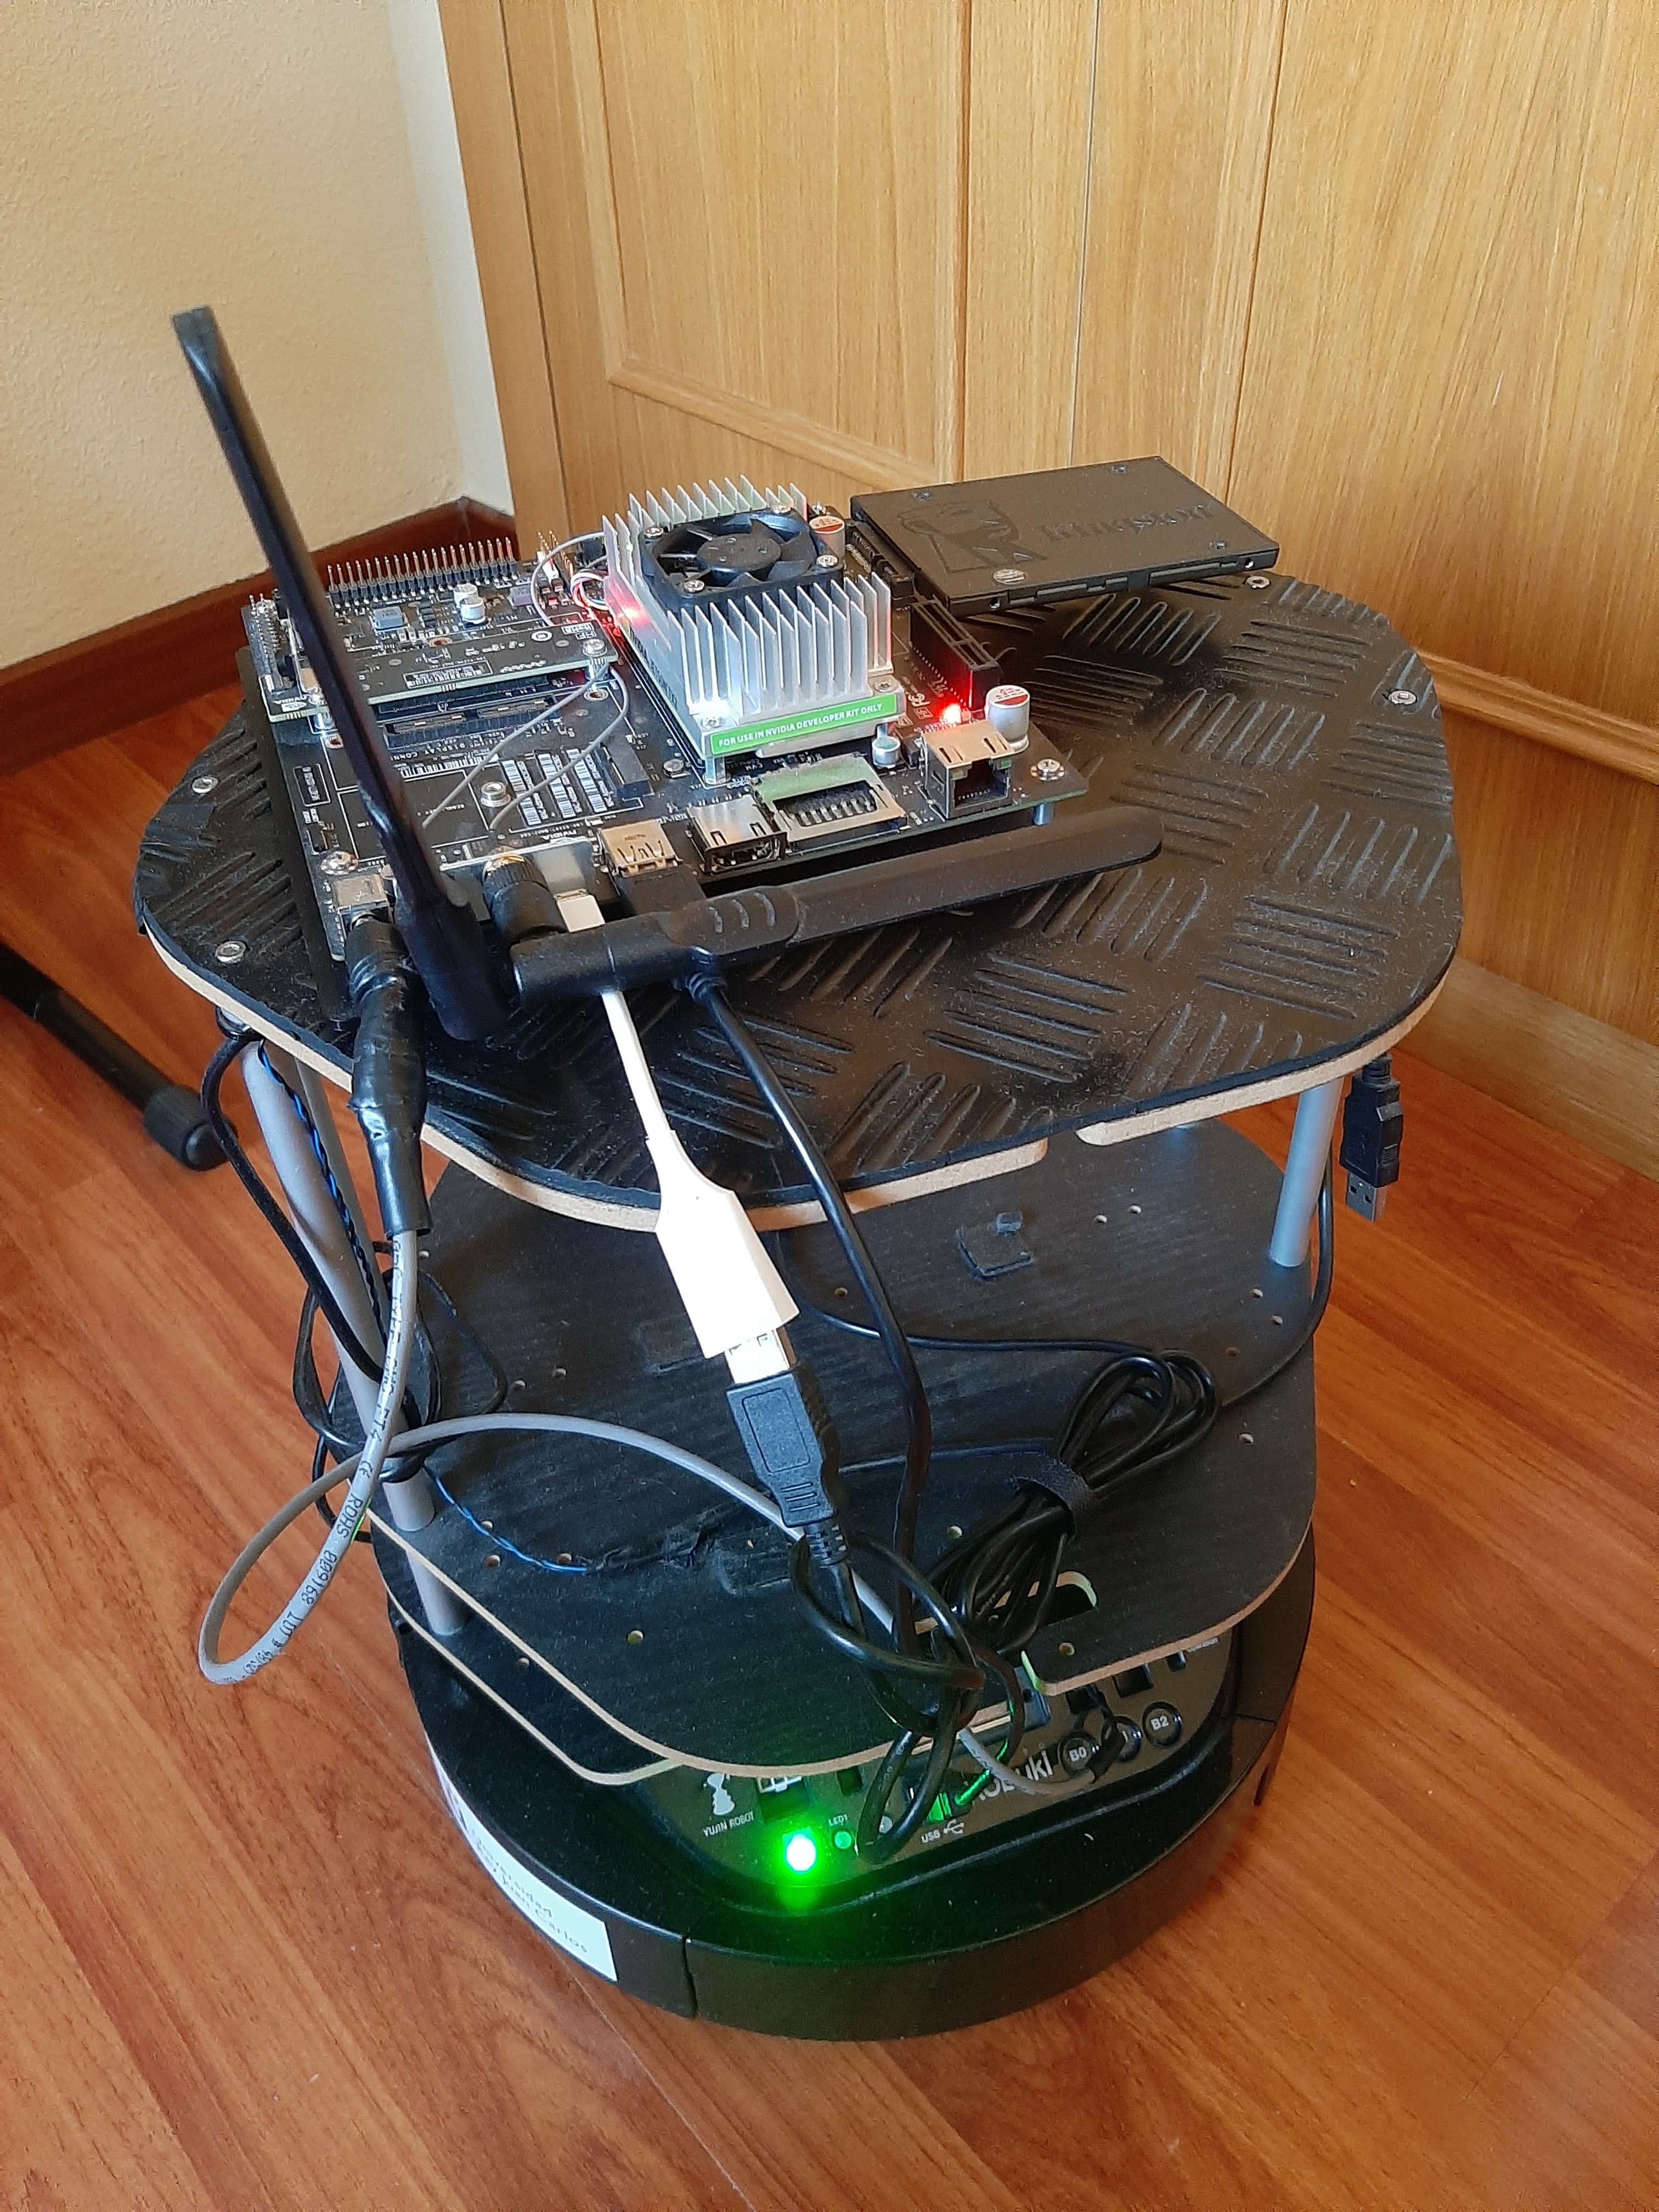
\includegraphics[width=0.9\linewidth]{setup_rear}
		\caption{Rear view.}
	\end{subfigure}
	\caption{Autonomous setup: Turtlebot2 + Jetson TX2 + ASUS Xtion Pro Live.}
	\label{fig:2_setup}
\end{figure}


\section{Software}

The development of this solution has been tackled using exclusively open-source software. The Jetson computing board follows a tightly optimized embedded design guidelines, thus a tailored version of Ubuntu Linux, named NVIDIA JetPack, is developed and maintained by NVIDIA, and it is available for download and install as the board firmware. For the developed system, the version used is JetPack 4.2.2 (R32.2)\footnote{Details available on: \url{https://docs.nvidia.com/jetson/archives/jetpack-archived/jetpack-422/release-notes/index.html}}. This custom implementation includes low-level interfaces for implementing parallel computing operations (CUDA), and several optimizations SDKs (\textit{Software Development Kits}), such as TensorRT. This engine is of special interest for us, as it allows to modify the underlying implementation of a neural network, swapping certain modules (such as a convolution operation, a ReLU, or an Inception block), for a low-level optimized version of that module, allowing to greatly increase the inference speed without entailing a precision loss. Several details about these optimizations will be depicted later.\\

Another remarkable difference is the Python implementation of this work. The version developed on \cite{tfg} was written using Python 2, and the ROS robotics middleware on its Kinetic release. However, both Python 2 and ROS Kinetic reached the EOL (\textit{End-Of-Life}) for the time this work has been revisited. Thus, the entire framework has been translated to Python 3.6, which is a currently supported release, as well as towards ROS \textit{Melodic Morenia}. Additionally, the image processing library OpenCV has been updated to the 4.x release. These changes, besides the fact that the Jetson TX2 board is based on an ARM architecture, has required several tweaks on the software compiling and implementation processes, which have been properly documented in the project repository\footnote{\url{https://github.com/RoboticsLabURJC/2017-tfg-nacho_condes}} for the sake of repeatability.\\

As in the previous work, the deep learning framework used is TensorFlow, bringing in a binding component called \texttt{TensorFlowRT/TRT}, used to implement the low-level optimizations on the TensorFlow neural engines.



\section{Functional architecture}
The software implemented in this work has been split into two main components or modules, namely the \textit{perception} module and the \textit{actuation module}, which can be observed in \autoref{fig:2_functional_architecture}.

\begin{figure}[h]
	\centering
	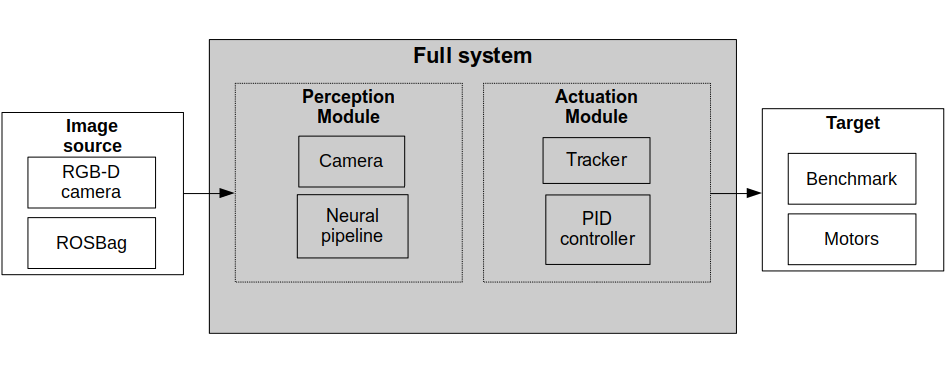
\includegraphics[width=0.7\linewidth]{functional_architecture}
	\caption{Functional architecture of the developed work, showing the two main blocks.}
	\label{fig:2_functional_architecture}
\end{figure}

These two modules cope with specific tasks on an independent manner, as it will be depicted in the following subsections:

\subsection{Perception Module}
This module encompasses what the robot perceives from its sensors (the camera, in this case), and the processing performed to the images in order to determine the location of the person to be followed.
\subsubsection{Camera}
As it was described before, the Xtion device yields two simultaneous images: an RGB image and a depth image. The ROS controller for the camera, OpenNI2\footnote{\url{https://structure.io/openni}}, fetches the image and registered depth map from the camera, making this information available through several ROS topics. As ROS follows a \textit{publisher-subscriber} semantics, once the driver is up and running, any application can subscribe to the topics in order to receive all the published messages. In our \textit{Camera} module, two subscribers are deployed to retrieve the latest (RGB, depth) pair on an asynchronous way. These images are then converted into the standard image format in the OpenCV library, and they are ready to be used by other components. Additionally, in order to be able to perform objective testing and benchmarks, these images can be read as well from a \textit{ROSBag}, which is a file containing a record of the messages published in specific topics for the time while it was recording. If a bag records the topics served by the camera driver, playing back the bag later allows to recover the messages (hence, the images) that were recorded by the camera previously. This allows to test different parameters under the same exact conditions, as the image sequences are now repeatable, as the ROSBag can be seen as a \textit{video sequence} of the image and depth topics (the recorded topics can be freely configured in the moment of recording the bag).\\

The implemented \textit{Camera} module abstracts this condition, allowing to apply the system on an \textit{online} source (camera) or an \textit{offline} source (recorded ROSBag), on a transparent adaptation to the rest of the system. Whenever a new (RGB, depth) pair is required, the \textit{Camera} module will serve the latest available image from the specified source.\\

\subsubsection{Neural pipeline}

On the other hand, the received images are passed through an ensemble of neural networks, which provide the capability of detecting the persons in the scene, as well as identifying which one is the one to be followed. As it was studied in \autoref{sec:1_sota}, the most powerful approaches are achieved nowadays using deep learning. Thus, the complex problem of determining the identity and location of the person of interest has been decomposed into three tasks, which are addressed using deep learning techniques:
\begin{description}
	\item[Person detection] the generalized \textit{object detection} task (\autoref{fig:2_person_detection}) is a commonplace challenge in computer vision. The existing solutions use object detectors similar to those explained in \autoref{sec:1_sota}, which are typically trained in large image datasets. The classes these models are capable to detect contain the \textit{person} class. Thus, as it was demonstrated in \cite{tfg}, a deep object detector can be utilized for detecting persons inside the image. On this work, several models have been tested, varying the base network architecture and depth. As one of the objectives of the system is to work on a portable (low-power) system, only the architectures which yield a good performance with a sufficiently low inference time are considered. The two most suitable models for this purpose are SSD \cite{ssd} using a MobileNet \cite{mobilenet} for feature extraction, and YOLOv3 \cite{yolov3} on its tiny version. These models are previously trained and publicly available on the TensorFlow Model Zoo\footnote{\url{https://github.com/tensorflow/models/blob/master/research/object_detection/g3doc/detection_model_zoo.md}} and on repositories hosted on GitHub\footnote{\url{https://github.com/mystic123/tensorflow-yolo-v3}}. In-depth testings have been developed to compare the performance of these two models, which can be found in \autoref{chap:3_results}. The previously developed work \cite{tfg} only supported SSD-based detectors, however, the object detection component of the program has been upgraded and it features YOLOv3 support as well, making it available through the configuration file specified on launch.
	
\begin{figure}[h]
	\centering
	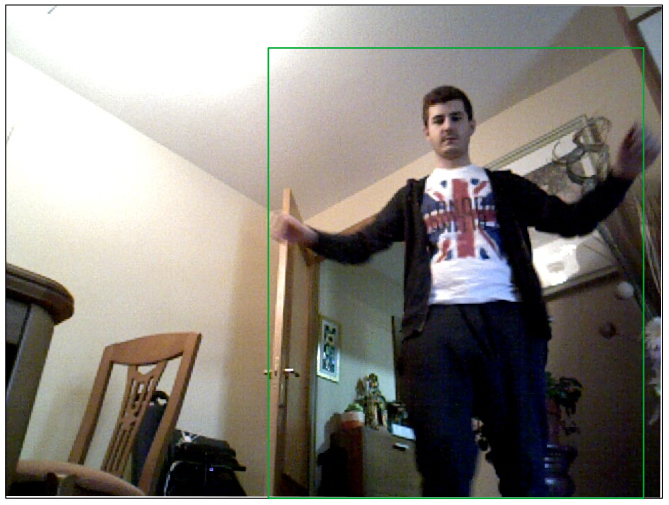
\includegraphics[width=0.5\linewidth]{person_detection}
	\caption{Example of a person detection task.}
	\label{fig:2_person_detection}
\end{figure}
	
	\item[Face detection] as in the previous point, the problem can be addressed using an object detection neural network. However, the previously deployed models are not capable of detecting faces. As the system is power-limited, looking for another multi-class model could be considered as an overshooting solution that the system is not able to handle at the same time the other model is deployed. Thus, one feasible solution is to use a single-class detection system. The network trained in \cite{faced} implements a two-stage neural network capable of detecting faces. As it was depicted in \autoref{sec:1_sota}, this detector is based on YOLO, which ensures a high-speed and efficient detection deployed using a class-specific neural network, which is way lighter than a multi-class detection system. The repository where the project is hosted contains a video sequence comparison comparing the precision of this system against a classical Haar cascade approach \cite{violajones}. \autoref{chap:3_results} contains captions of this sequence to show the superior performance for the face detection issue.
	
	\item[Face identification] Once the face of a person has been retrieved, it can be used as a distinguishing feature for determining their identity. As the basis of this work is to take advantage of deep learning power, a neural system has been selected to perform this task. For this purpose, the described system \textit{FaceNet} has been deployed in order to perform identification, using a publicly available implementation in TensorFlow\footnote{\url{https://github.com/davidsandberg/facenet}}. As a result, we can transform the image of a face into a 128-dimensional vector: its projection or \textit{embedding}. This transformation is learned after a triplet-loss training process, which separates different faces as much as possible, while projecting similar faces as close as possible. As it can be seen on \autoref{fig:1_faces_poses}, we can use this method to obtain similar projections when two images of the same face are evaluated, despite different lighting conditions (as a channel-wise normalization step is performed before passing the image through the network).
	
\end{description}

To sum up, this ensemble of 3 neural networks provides a sequential pipeline to obtain \textit{person locations, face detections and face projections} from a single image, taking advantage of the flexibility that deep learning methods offer, in order to address three different problems on an efficient way.\\

Once the inference pipeline has been designed and implemented, we can take advantage of the optimization libraries present in the Jetson TX2 board, using TensorRT for this purpose. Using this library, several segments from the architecture of a given network can be modified according to certain parameters:

\begin{description}
	\item[MSS (\textit{Minimum Segment Size})] the threshold above which a segment is selected to be replaced by the TensorRT optimization. Increasing this value makes the optimizer more selective, in order to optimize only the heaviest segments of the network. 
	\item[MCE (\textit{Maximum Cached Engines})] TensorRT keeps a cache of engines on runtime, with the purpose of reducing the time spent for loading them into the GPU. This parameter modulates the amount of engines kept in that cache, in case the available memory to establish the cache is limited.
	\item[Precision mode] typically, the weights and parameters of the trained neural networks are handled as 64-bit floating point numbers. A reduction in the precision to 32-bit or 16-bit achieves very similar results, making the operations much lighter as the precision mode is reduced by $\frac{1}{2}$ or $\frac{1}{4}$. A more daring approach reduces the precision up to 8-bit integers, performing an additional \textit{quantization} step since the range will be limited to 256 values. The quantization step analyzes the segment, computing the numeric range of its weights. This range is typically narrow enough to perform a 8-bit quantization, mapping the high-precision weights into a range composed of 256 values between the minimum and maximum values of the weights.
\end{description}

An experimental tuning of these parameters has been performed in this work, looking for an optimization of the inference time and taking into account that the enhanced models of the three neural networks have to share the limited memory on board. Thus, care has to be put into the memory footprint that an excessive runtime optimization might cause, as this leads to a high time penalization if the system cache is utilized to store the models.\\


The \textit{Camera} and \textit{Neural} components form the \textit{Perception} module, responsible of retrieving the external image and apprehend the underlying information from the image: position and identity of the person to be followed.


\subsection{Actuation Module}

The second module of the system addresses the actuation task: once the external stimuli have been acquired and processed, an action has to be performed in order to move the robot towards its goal. As the final objective of the system is to follow a person, these movements have to be reactive, happening as soon as possible whenever the person changes her position.\\

\subsubsection{Motion Tracker}

The previously depicted \textit{Neural} module outputs trustworthy inferences with a certain refresh rate, namely $K$, which can reach a relatively high value depending on the current load and power profile in the development board. If $K$ is too high, the system can run the risk of suffering an important delay when the movement is performed. This can lead in unsteady movements, with a higher probability of losing the reference person. To avoid this, a \textit{Tracker} component is added to the system. Its functionality is to be able to \textit{estimate} the person movement during $K$ frames, while the neural pipeline is performing detections. This way, currently detected persons can be tracked along the image while they wander, until the neural ensemble outputs the latest predictions, which determine the true new position of the persons. To fulfill this requirement, the tracking method has to be able to run at a higher rate than $K$, preferably with a considerably lower inference time. This way, the system counts on a slow, reliable detection system supported by a fast estimation system, devoted to guess the movements between detections.\\

The method chosen for this purpose is a \textit{Lucas-Kanade} visual tracker\cite{diapos_cv_motion_estimation}.  This technique estimates the \textit{motion field} between the images taken in two time instants, addressing the problem using a differential approach\cite{lucas_kanade}:

The basis relies on the fact that in a video sequence, for small changes in space and time, the intensity remains constant inside a certain pixel neighborhood:

$$
\mathbb{I}(\mathbf{x}, t) = \mathbb{I}(\mathbf{x} + \Delta \textbf{x}, t + \Delta t)
$$

Using a \nth{1} order Taylor series approximation and algebra, the \textit{optical flow equation}, $f$, can be found\cite{lucas_kanade_tutorial}:

$$
f_xu+ f_yv + f_t = 0
$$
where
$$
f_x = \frac{\partial f}{\partial x} ; f_y = \frac{\partial f}{\partial y}\\
$$
$$
u = \frac{dx}{dt} ; v = \frac{dy}{dt}
$$

$f_x$, $f_y$ and $f_t$ represent the image gradients with respect to the space and time, respectively, and $(u, v)$ represents the movement vector of the scene.

\begin{figure}[h]
	\centering
	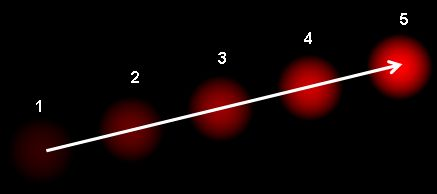
\includegraphics[width=0.6\linewidth]{optical_flow}
	\caption{Optical flow for different time instants. Image from \cite{lucas_kanade_tutorial}.}
	\label{fig:2_optical_flow}
\end{figure}

At this point, the resulting system is under-determined as the problem presents 1 equation with 2 unknown variables. Lucas-Kanade addresses this problem taking advantage of one of the previous assumptions: as the pixel intensity remains constant for a pixel neighborhood, one can expect the same movement on neighboring pixels: these will share a common $(u, v)$ movement vector (typically, a small square or circular neighborhood is assumed). Assembling together those equations results in an over-determined system, where a \textit{Least-Squares} solution yields the best-fitting movement vector $(u,v)$ for that neighborhood, allowing to have a local estimation for the movement in that area:

\begin{equation}
\begin{bmatrix} u \\ v \end{bmatrix} = \begin{bmatrix} \sum_{i}{f_{x_i}}^2 & \sum_{i}{f_{x_i} f_{y_i} } \\ \sum_{i}{f_{x_i} f_{y_i}} & \sum_{i}{f_{y_i}}^2 \end{bmatrix}^{-1} \begin{bmatrix} - \sum_{i}{f_{x_i} f_{t_i}} \\ - \sum_{i}{f_{y_i} f_{t_i}} \end{bmatrix}
\label{eqn:2_lk_ls}
\end{equation}

The computation of \autoref{eqn:2_lk_ls} can be efficiently performed with high-performance libraries, such as \textit{NumPy} or \textit{TBB}, which ensure a fast execution of the estimation. This makes Lucas-Kanade estimation an efficient approach to compute the optical flow in tasks such as image registration, video stabilization or depth computation in stereo vision systems. This technique is implemented in the \textit{OpenCV} library through the method\\ \texttt{cv2.calcOpticalFlowPyrLK}, which evaluates the image on a pyramid of scales to improve the robustness. This method offers a set of tunable parameters to detect the corners:

\begin{description}
	\item[\texttt{winSize}] size of the window to perform the LS solution.
	\item[\texttt{maxLevel}] number of additional scales to evaluate the image on a pyramidal scale sequence.
	\item[\texttt{criteria}] flags to determine the stop condition on the iterations of the algorithm.
\end{description}

However, in the case of study of this work, a calculation of the motion field on the entire image would be considered overshooting (besides of a dangerously slow task for a real-time system), as the objective is not to compute the entire optical flow. The estimation can be limited to the pixels inside and surrounding the persons in the scene. Furthermore, one can notice the existence of more informative regions inside the person than others, given its texture: typically object \textit{corners} will be the best choice to be tracked \cite{diapos_cv_features}, given their easiness to be identified and the fact that they provide more motion information than another areas (aperture problem). In order to detect these corners, a Harris corner detector can be used, analyzing the eigenvalues inside different 2-D windows inside the image. A \textit{corner response} can be computed, yielding a score depending on the eigenvalues and their ratio:
$$
R = \det M - k(\operatorname{trace}(M))^2
$$
with k being an empirical constant $k=0.04-0.06$, and $M$ being the diagonal matrix resulting of the singular value decomposition of the current window.

The value of $R$ determines the decision taken of the window containing a corner.

A modification of this algorithm, the \textit{Shi-Tomasi} corner detector was published on \cite{shi_tomasi}, improving the performance of the corner detector by changing the corner response computation to:
$$
R = \min(\lambda_1, \lambda_2)
$$

taking the window as a corner if $R$ is greater than a given threshold. The scoring diagrams for determining the corner response on the two depicted methods can be observed in \autoref{fig:2_harris_vs_shi}. One advantage of this methodology is its invariance to rotation, as it works using the eigenvalues, that automatically align to the most variant directions. However, one important thing to mention as a flaw is the variance to scale: the relative size of the corner with respect to the window size has influence on the eigenvalues 

\begin{figure}[h]
	\centering
	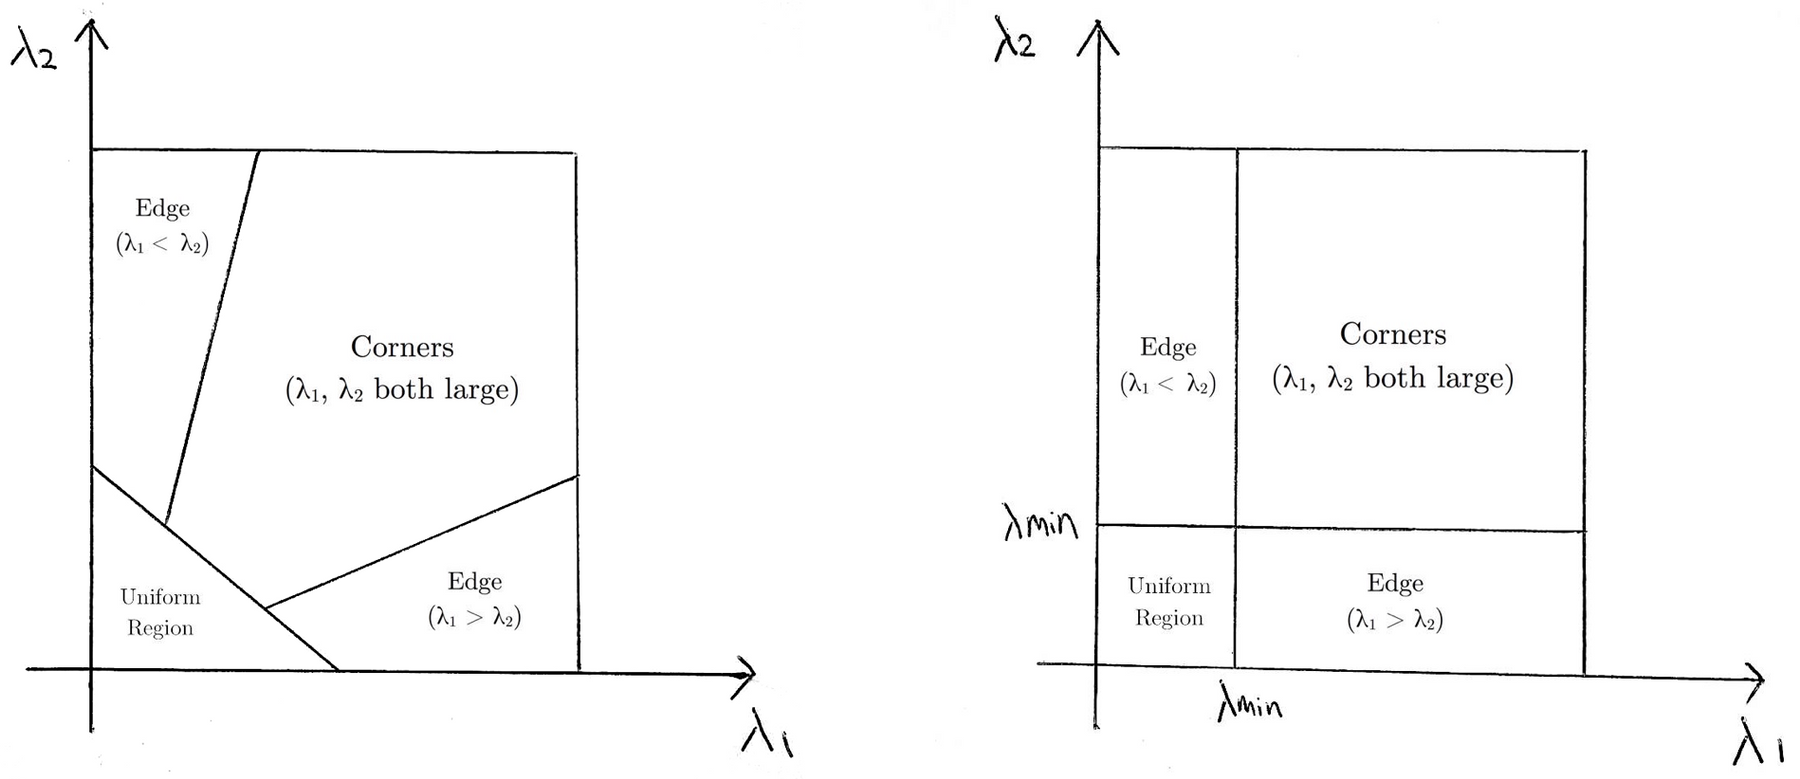
\includegraphics[width=0.8\linewidth]{harris_vs_shi_boundaries}
	\caption{Corner response $R$ scoring functions on $\lambda_1-\lambda_2$ on the Harris (left) and Shi-Tomasi (right) detectors (source:\cite{nanonets_optical_flow}).}
	\label{fig:2_harris_vs_shi}
\end{figure}

\begin{figure}[h]
	\centering
	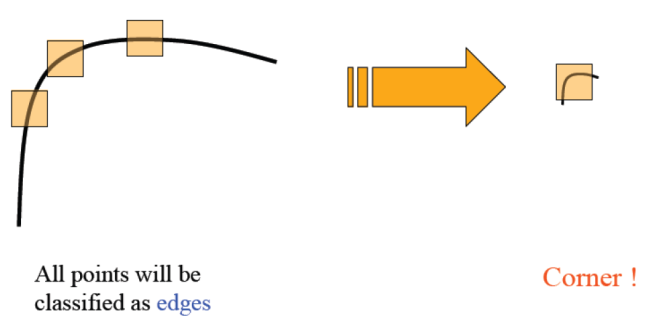
\includegraphics[width=0.8\linewidth]{harris_scale_variance}
	\caption{Scale variance of this method, where the size of the corner with respect to the \texttt{winSize} jeopardizes the eigenvalues.}
	\label{fig:2_harris_scale}
\end{figure}

Using this method returns what the authors call the \textit{good features to track}, namely, the best N corners of the image or region provided.

 This method is implemented in the \textit{OpenCV} library through the method \texttt{cv2.goodFeaturesToTrack}, which offers a set of tunable parameters to extract corners from a given image:
 \begin{description}
 	\item[\texttt{maxCorners}] maximum number of corners to be found.
 	\item[\texttt{qualityLevel}] multiplicative factor for the $R$ of the best corner. A corner response below $\text{qualityLevel}\cdot R_{max}$ will be discarded.
 	\item[\texttt{minDistance}] minimum euclidean distance between the selected corners.
 	\item[\texttt{blockSize}] size of the pixel block to compute the eigenvalues.
 \end{description}

The combination of these two methods provides a fast methodology to estimate the movement of a region using exclusively algebraic calculations on the pixel intensities. As these computations are bounded in complexity, the iteration time is around 5x faster than the neural pipeline. Thus, the simultaneous combination of both algorithms allows to track the movements of the persons during $K$ frames, until the next neural update arrives. This is shown in \autoref{fig:2_tracker_demo}.\\

\begin{figure}[h]
	\centering
	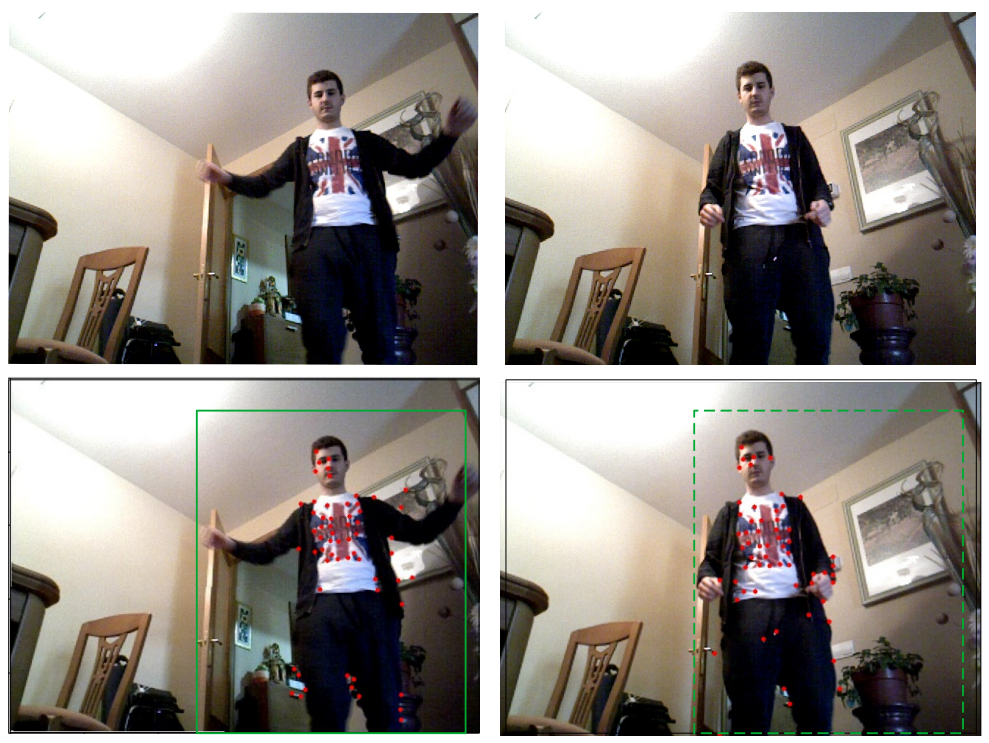
\includegraphics[width=0.9\linewidth]{tracker_demo}
	\caption{Operation of the tracking module: the last detection (green) determines the person position. The keypoints (red) are tracked during $K$ frames until the next neural update.}
	\label{fig:2_tracker_demo}
\end{figure}

As the \textit{OpenCV} implementation of Lucas-Kanade identifies the points that have been found in both frames, the average displacement of all the points can be computed. This allows to displace the bounding box of that person using the computed displacement vector. Additionally, it can be rescaled in case the person moves closer or further from the camera, using the distribution of the points in the previous and current frame. As it can be seen on \autoref{fig:2_tracker_update}, the Shi-Tomasi corner detector finds a set of corners (keypoints) in the frame $t$, drawn with red points. These points are distributed with a given mean: , the centroid of the cloud, represented with an "x", beside of a standard deviation pair ($\sigma_x^t, \sigma_y^t$). On the next frame, some new keypoints are found (green), whereas keypoints from the previous frame are identified. These points are useful for computing the new centroid ($\mu_x^{t+1}, \mu_y^{t+1}$) and deviations pair ($\sigma_x^{t+1}, \sigma_y^{t+1}$). With this information, the person box can be updated accordingly:

\begin{align*}
&\text{person\_coordinates}(t) = \left[\mu_x^{t}, \mu_y^{t}, w, h\right]\\
&\text{person\_coordinates}(t) = \left[\mu_x^{t+1}, \mu_y^{t+1}, w\cdot\frac{\sigma_x^{t+1}}{\sigma_x^t}, h\cdot\frac{\sigma_y^{t+1}}{\sigma_y^t}\right]\\
\end{align*}

\begin{figure}[h]
	\centering
	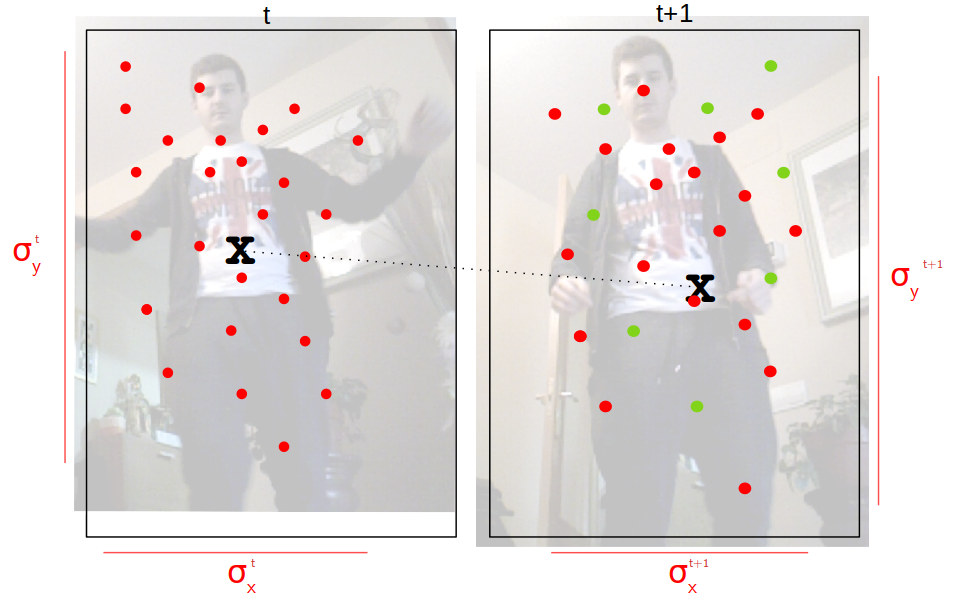
\includegraphics[width=0.9\linewidth]{tracker_update}
	\caption{Update of the Lucas-Kanade tracker from frame $t$ to frame $t+1$.}
	\label{fig:2_tracker_update}
\end{figure}

This way, the update is sensitive to displacements and scale changes in both directions, in case the person changes her linear distance to the camera.\\



Its introduction enhances the robustness as the output of the system will not depend just on the neural detections. This improves the performance as partial occlusions might cause some detections to be discarded momentarily. The introduction of the tracker can palliate this effect, as the person will be kept as \textit{detected} for a number of frames even if it is not detected by the neural pipeline, and its position will be tracked using Lucas-Kanade. This number of frames is called \textit{patience}, $P$, and introduces an hysteresis in the tracker, as a person has to be lost for $P$ frames in a row to be discarded.\\



On the same way, a detection has to be maintained during $P$ frames to be joined to the tracked persons. The patience component is introduced in pursuit of stability in case the scenario complicates a stable detection. In such cases a detection flickering is observable, and this could lead in an erratic movement on the robot. The introduction of the patience solves this problem successfully.


\subsubsection{PID Controllers}
The combination of the described systems results in a efficient way to detect and identify the person to be followed, and additionally, track her movements on a fast way between slower detections.\\

The last block of the system is responsible of  translating this location information of the reference person into velocity commands that move the robot towards an \textit{acceptable position} with respect to the person, where certain conditions are fulfilled.\\

As it was described on \autoref{sec:2_materials}, the robot offers 2 degrees of freedom: rotation speed and linear speed. Thus, this \textit{acceptable position} can be described in those 2 dimensions:
\begin{description}
	\item[Angular position] the reference person has to be placed at a side angle of 0º with respect to the robot front.
	\item[Linear position] the reference person has to be placed at a distance of 1 m with respect to the robot front.
\end{description}

Due to the sensors uncertainty, the prediction and tracking estimation, and the movements of the person, these positions have to be extended to \textit{safe areas}, inside of which the robot will not trigger a velocity command for that dimension. This is achieved introducing a \textit{margin/tolerance} on each dimension. Additionally, these geometric criterion have to be translated to measurable discrepancies. This way, the safe zones can be defined as:

\begin{description}
	\item[Angular zone] the reference person has to be placed at the horizontal center of the image, with a margin of $\pm 50$ pixels on the sides.
	\item[Linear zone] the reference person has to be placed at a distance of 1 m with respect to the robot front, with a distance margin of $\pm 30$ cm\footnote{This criteria can be maintained in metric distance, as the depth sensor specifically yields that information. In the angular case, the image is a 2D projection on the camera plane, which does not allow to infer the relative angle with the person without extra computations using the relative distance.}.
\end{description}

These regions, which are completely tunable using the configuration file, can be visualized on \autoref{fig:2_velocity_controllers}.

\begin{figure}[h]
	\centering
	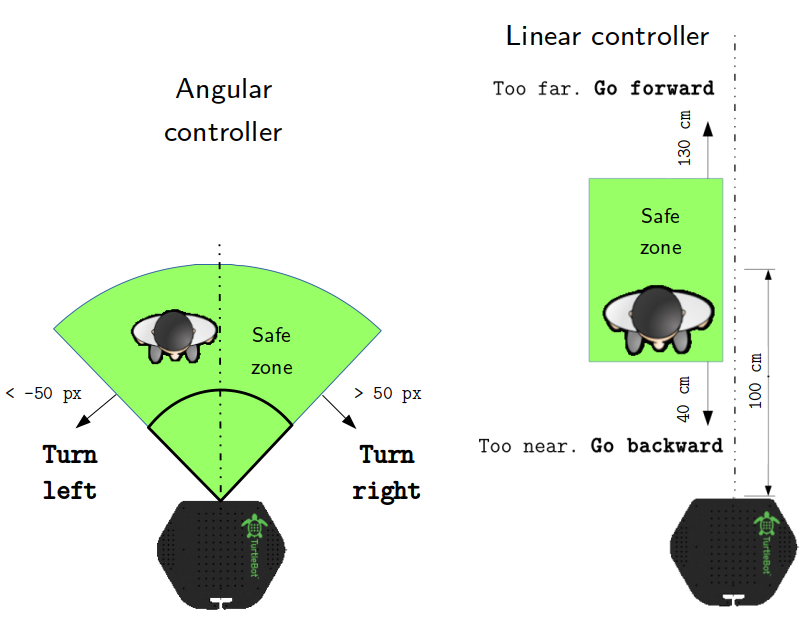
\includegraphics[width=0.7\linewidth]{velocity_controllers}
	\caption{Safe zones for each controller. Image from \cite{tfg}.}
	\label{fig:2_velocity_controllers}
\end{figure}

To place the person inside these safe zones, the robot has to move on certain directions. For determining a movement, an \textit{error} vector ($e_x, e_w$) is computed, using the tracked person coordinates:

\begin{description}
	\item[$e_x$] the linear error or \textit{range} is computed using the depth image, estimating the distance from the robot to the person. As the Xtion sensor registers the depth image into the RGB one, the person coordinates can be used in the depth image in order to find the distance of each pixel inside the bounding box of the reference person: the \textit{person depth map}. As it is feasible that the box contains an important region of the background (specially if the person opens her arms, as the neural detection will encompass the entire body), the edges of the depth map are trimmed. Later, a 10x10 grid is computed to have 100 uniformly distributed samples of the depth of the person. In order to ensure that the background does not affect the range measurement, the median value is computed, as even if some outlier points belong to the background, they would have to make up the 50\% of the sampled set to deviate the measurement from the true range.
	
	\item[$e_w$] the angular error can be computed taking into account that if the robot and the person are aligned, its bounding box will be horizontally placed near the center of the image. Therefore, an error metric can be extracted computing the difference on the horizontal coordinate between the image center and the center of the bounding box of the reference person.
\end{description}

These computations can be visualized on \autoref{fig:2_controller_error_computation}.


\begin{figure}[h]
	\centering
	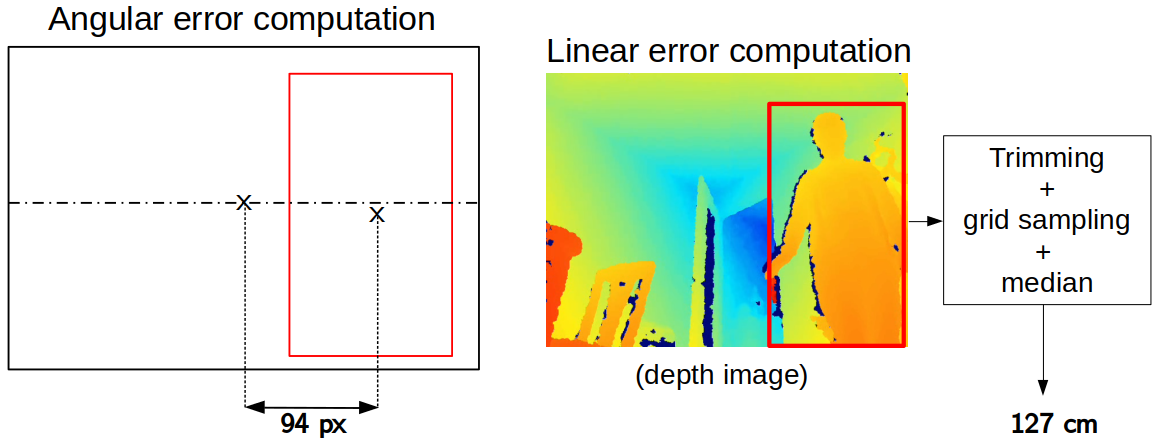
\includegraphics[width=0.95\linewidth]{controller_error_computation}
	\caption{Error computation on each controller.}
	\label{fig:2_controller_error_computation}
\end{figure}

The last step of the controller takes care of computing two proper response (linear and angular) for the robot. If these responses depend only on the error readouts, the robot might receive unsteady commands, that might cause a total loss of the person from the field of view. This can be solved introducing a slightly more complex system: a PID controller \cite{pid_controllers}, which is a closed-loop control system that outputs a response taking into account the previously sent responses.\\

The \textit{PID} acronym stands for \textit{Proportional, Integral and Derivative}, as that is the methodology followed to output a response. The output in the time instant $t$, $u[t]$ depends on the currently measured error, $e[n]$, and it is computed as follows: 

\begin{equation}
u[n] = k_p e[n] \ \ + \ \ k_i \sum_{i=0}^{n}e[i] \ \ + \ \ k_d (e[n] - e[n-1])
\label{eq:6_pid}
\end{equation}
This equation can be split into the three components:
\begin{description}
	\item[Proportional] $k_p e[n]$. This is the basic component, that computes a response directly proportional to the measured error.
	\item[Integral] $k_i \sum_{i=0}^{n}e[i]$. An additional response, equivalent to the sum of the total error until the current instant. This way, although a proportional response is not enough and the error gets stabilized in a non-zero value, the system will accumulate that error, increasing the response magnitude in order to close the existing gap between the error and the desired readout\footnote{When the monitored variable goes into the tolerated zone again, the total error has to be reset, as it is not required from now on.}.
	\item[Derivative] $k_d (e[n] - e[n-1])$. This part stands for the \emph{difference} between the last measured error and the current one, and it quantifies how is the system responding\footnote{On systems without inertia, this contribution is generally ignored, having a simple PI control loop instead.}. If the difference has a high value, that means that the system is on a far state/position with respect to the last iteration. So, in order to eliminate the \emph{inertia} the system could have acquired (which might bring oscillations and overshooting), the derivative part acts, braking or accelerating the command depending on the observed response to the previous one.
\end{description}




\autoref{fig:2_pids} shows that the combination of the three sub-responses can achieve a fast and steady response (\autoref{fig:2_pids}), bringing back the system under control on an efficient way.

\begin{figure}[h]
	\centering
	\begin{subfigure}[b]{0.3\linewidth}
		\centering
		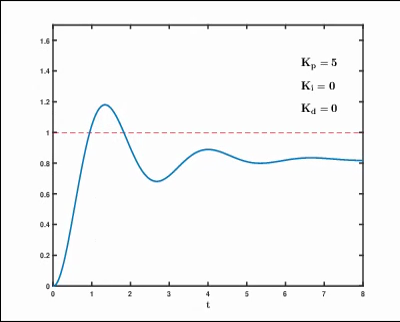
\includegraphics[width=\linewidth]{pid_p}
		\caption{Proportional.}
		\label{fig:2_pid_p}
	\end{subfigure}
	\hfill
	\begin{subfigure}[b]{0.3\linewidth}
		\centering
		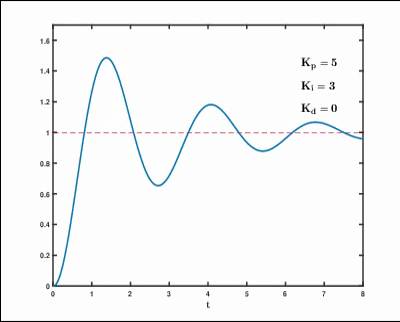
\includegraphics[width=\linewidth]{pid_pi}
		\caption{PI.}
		\label{fig:2_pid_pi}
	\end{subfigure}
	\hfill
	\begin{subfigure}[b]{0.3\linewidth}
		\centering
		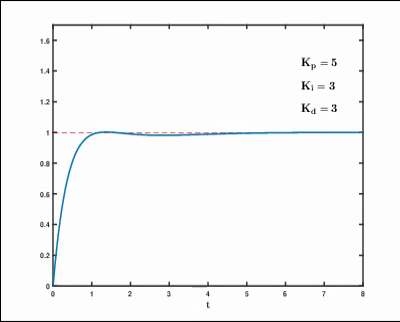
\includegraphics[width=\linewidth]{pid_pid}
		\caption{Full PID.}
		\label{fig:2_pid_pid}
	\end{subfigure}
	\caption{Different controllers response along time.}
	\label{fig:2_pids}		 	
\end{figure}

Each contribution is parameterized by its corresponding constant ($k_p, k_i, k_d$), so a task to perform is to find the optimum value for each one of them. Visual assessments of the robot stability under different combinations lead to the values present in \autoref{tab:2_pids}, which yielded a steady behavioral of the robot when it is subject to typical indoor conditions of following a person wandering. As previous parameters, these values can be changed using the configuration file.

\begin{table}[h]
	\centering
	\begin{tabular}{|c|c|c|}
		\hline
		\textbf{} & \textbf{Linear} & \textbf{Angular} \\ \hline
		$k_p$     & 0.4               & 0.005               \\ \hline
		$k_d$     & 0.04              & 0.0003              \\ \hline
		$k_i$     & 0.05              & 0.006               \\ \hline
	\end{tabular}
	\caption{Optimal found values for the parameters in each PID controller.}
	\label{tab:2_pids}
\end{table}

Finally, when the speed is computed, it is adapted to a ROS message, and it is published to the topic devoted to velocity commands to the robot. On the other side of the topic, the driver reads these messages and moves the robot accordingly with the commands received.\\

This last block completes the functional architecture of the full following system.

\section{Software architecture}

The developed software puts all the previous components together, offering two application modes:
\begin{description}
	\item[\texttt{followperson} mode] this is the default behavioral of the system. When running on this mode, the program feeds the tracker and the neural pipeline with images from the ASUS Xtion, and sends the velocity commands to the robot, writing them into the specified ROS topic.
	
	\item[\texttt{benchmark} mode] this mode is designed to test the entire infrastructure, with the purpose of tuning parameters or extracting objective metrics for comparisons, such as precision, or inference time. The images are read from a previously recorded ROSBag, emulating the Xtion sensor and providing always the same RGBD sequence to be fed in different implementations, allowing to compare the performance of different configurations under identical conditions. On this mode, the velocity commands are not sent to the robot, just drawn in the output image (\autoref{fig:2_output_image}), which is also saved into an output video for later visualization. Aside of the video, execution graphs and YAML\footnote{YAML is a plain-text data serialization format. It has been chosen as a standard format on this project as it offers a good tradeoff between serialization (allowing the data to be converted back into data structures in Python) and  readability of the file without processing it.} files are stored containing information about the tracked persons and times for each frame processed by the \texttt{Main} thread.
\end{description}

This behavioral, and other parameters, can be configured on the program execution without modifying the source code. The program receives a YAML configuration file specifying all the required parameters in order to run the system:

\begin{lstlisting}
NodeName: "followperson"
Benchmark: true # true for benchmark, false for followperson
RosbagFile: "resources/bag1.bag"  # path to the ROSBag if benchmark 
LogDir: "resources/benchmarks" # where to write the results

Networks:
  # Parameters for the neural pipeline
  Arch: ssd # detection architecture [ssd, yolov3, yolov3tiny]
  DetectionModel: "models/ssd_mobilenet_v1_0.75_depth_coco.pb"
  DetectionWidth: 416 # usually 300 for SSD, 416 for YOLOv3tiny
  DetectionHeight: 416 # usually 300 for SSD, 416 for YOLOv3tiny
  FaceEncoderModel: "models/facenet_inception_resnet_vggface2.pb"

RefFace: "resources/ref_face.jpg" # Image of the reference face

Topics:
  RGB: "/camera/rgb/image_raw" # topic publishing the RGB images
  Depth: "/camera/depth_registered/image_raw" # topic publishing the depth images

# Parameters for the speed controllers
XController:
  Kp: 0.4
  Ki: 0.04
  Kd: 0.05
  Min: 0.7
  Max: 1

WController:
  Kp: 0.005
  Ki: 0.0003
  Kd: 0.006
  Min: -50
  Max: 50
# Parameters for the people tracker
PeopleTracker:
  Patience: 5
  RefSimThr: 1.0
  SamePersonThr: 60
\end{lstlisting}


The previously depicted structure can be implemented on the Jetson board using the programming language Python. As the tracking module has to run \texttt{threading} library. The deployed threads on the system are:

\begin{description}
	\item[Main thread] the purpose of this thread is to continuously draw the output image (shown in \autoref{fig:2_output_image} and explained below), and compute the errors and suitable responses, as well as sending them to the robot. One thing to notice about this thread is that it does not process all the frames in the sequence, as its rate depends on the drawing time and the computation of the response. It works asynchronously, fetching the latest frame from the \texttt{tracker} thread.
	
	\item[\texttt{networks\_controller} thread] this controller handles the 3 described neural networks, running sequential inferences on them. In the Jetson platform, these neural networks are deployed in the GPU of the board. Therefore, this thread can be seen as the one which interacts with the GPU in order to pass, retrieve and transform tensors from the networks.
	
	\item[\texttt{tracker} thread] as it was shown before, the tracker must inherently iterate at a higher rate than the neural infrastructure. However, including it in the main thread would be bad for its performance, as the speed would be limited by the image drawing and responses publication in the speed topics. Therefore, it is extracted to a devoted thread. The simplicity of the Lucas-Kanade tracker makes it fast to execute, however it would be pointless to track a person several times before a new image arrives from the camera. To avoid this, the thread has a rate limitation of 30 Hz, equal to the framerate of the Xtion sensor.\\
	
	As this is the fastest thread to execute, and it is crucial that the tracker has available every image from the camera, this is the first component to receive the images from the source, on a 30 Hz synchronous manner. The rest of components can fetch the images asynchronously from the tracker whenever they need them.
	
	\item[ROSCam] this component, responsible of fetching the images from the source (a ROSBag or the Xtion camera, as explained before) is not deployed as a thread. However, as it works by means of subscribers when a synchronous mode is required (thus, when the source is the Xtion camera), the ROS API for Python, \texttt{rospy} automatically deploys these subscribers on independent threads.
\end{description}

This software architecture can be seen in \autoref{fig:2_software_architecture}, where the behavioral interaction between the threads can be visualized. The \texttt{Main} thread varies its behavioral depending on the configured mode (\texttt{followperson}/\texttt{benchmark}), whereas the rest of threads  behave similarly in both configurations.

\begin{figure}[h]
	\centering
	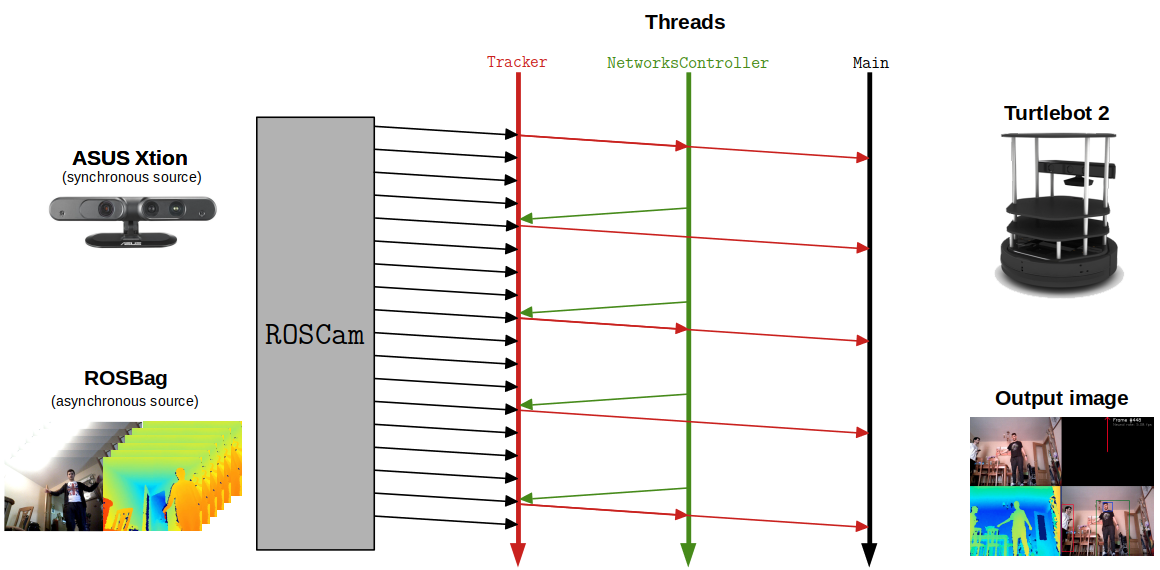
\includegraphics[width=0.8\linewidth]{software_architecture}
	\caption{Software architecture for the system.}
	\label{fig:2_software_architecture}
\end{figure}



The visible output of the system is the image shown in \autoref{fig:2_output_image}. This image is drawn by the main thread, when the position errors are computed and the responses have been sent to the robot, and it serves as monitoring means for the execution, showing the images, the tracked persons and the sent commands. If the benchmark mode is enabled, these image are appended to a output video, which serves for posterior visualization or assessments of the performance.

\begin{figure}[h]
	\centering
	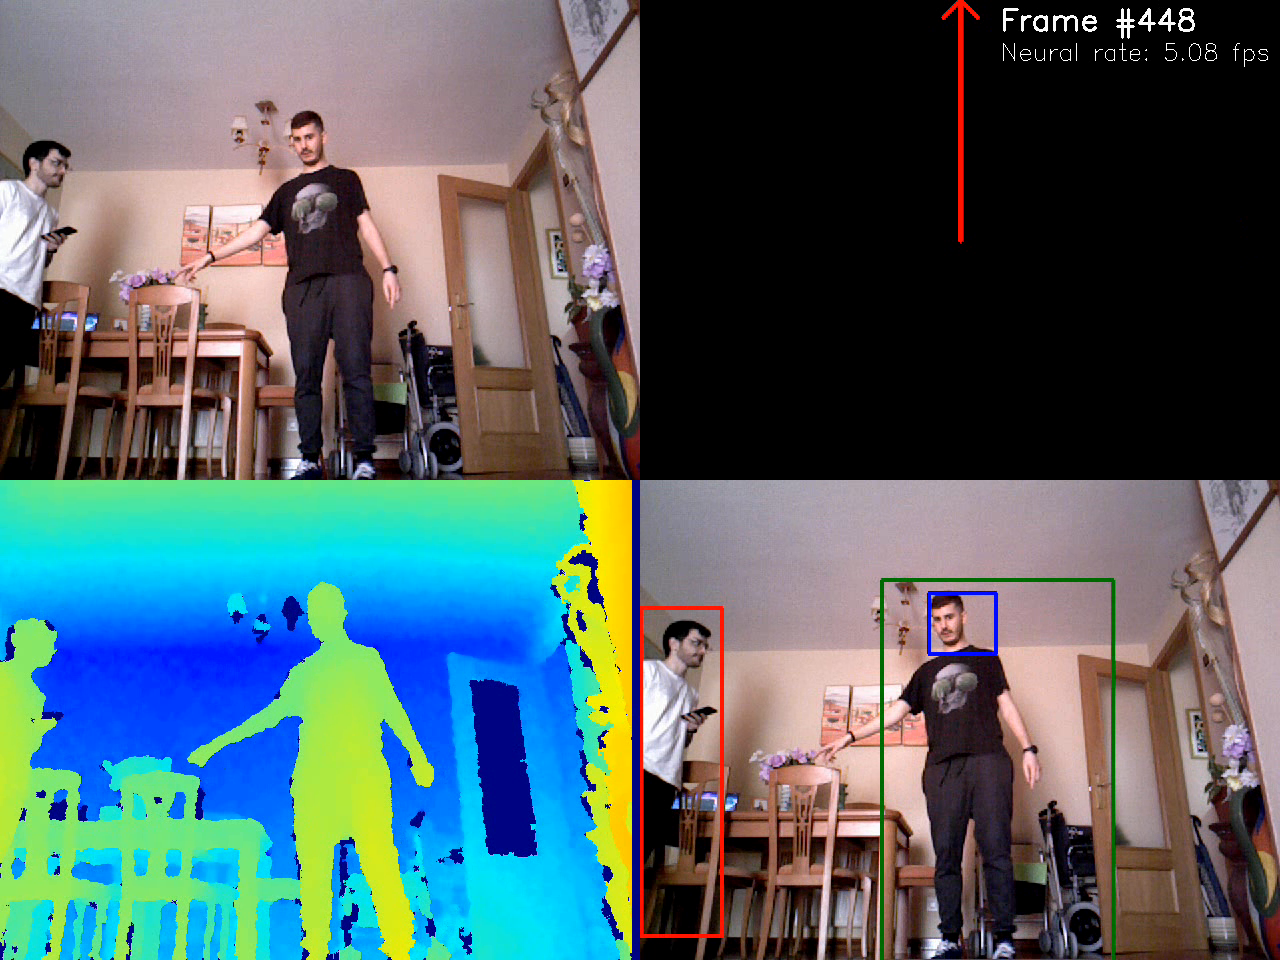
\includegraphics[width=0.85\linewidth]{output_image}
	\caption{Output image drawn by the program. Upper left: input RGB image. Bottom left: input depth image. Upper right: velocity commands sent to the robot, and information about the neural rate and number of current frame. Bottom right: tracked persons (green if it is reference, red otherwise) and their faces}
	\label{fig:2_output_image}
\end{figure}





%----------
%	BIBLIOGRAFÍA
%----------	

%\nocite{*} % Si quieres que aparezcan en la bibliografía todos los documentos que la componen (también los que no estén citados en el texto) descomenta esta línea

\clearpage
\addcontentsline{toc}{chapter}{Bibliography}
\printbibliography


%----------
%	ANEXOS
%----------	

% Si tu trabajo incluye anexos, puedes descomentar las siguientes líneas
%\chapter* {Annexes x}
%\pagenumbering{gobble} % Las páginas de los anexos no se numeran


\end{document}